\documentclass{article}
\usepackage{iclr2027_conference,times}

\usepackage{graphicx}
\usepackage{booktabs}
\usepackage{multirow}
\usepackage{rotating}
\usepackage{xcolor}
\usepackage{amsmath}
\usepackage{hyperref}
\usepackage{url}
\urlstyle{same}

\graphicspath{{figures/main/}{figures/appendix/}{figures/per-block-results/}{figures/methods/}{figures/results/}}

\title{Towards All-Atom Protein World Models: Learning and Diagnosing Predictive Latent Representations}

\author{Anonymous authors}
\begin{document}
\maketitle

\begin{abstract}
All-atom protein models compress atomic structure into latent representations, often using reconstruction or generative objectives that require these latents to preserve precise coordinate information. Yet, residue properties depend on both local atomic environments and longer-range 3D interactions. Joint-Embedding Predictive Architectures (JEPAs) offer an alternative: predicting representations in latent space rather than reconstructing the raw input. In vision, this shifts learning away from pixel-level reconstruction toward higher-level features that transfer across tasks. We ask whether the same approach can help protein representations capture both residue-level information and broader structural context useful for protein structure and function tasks. Using the La-Proteina encoder, we train JEPA, JEPA+SIGReg and LeJEPA on masked protein structures and evaluate them with StructTokenBench. We study how masking, positional information, rotations and cropped views affect the learned representations. JEPA with 70\% random masking scores higher than the C$\alpha$-conditioned La-Proteina baseline on 17 of 21 functional-site and flexibility scores. In JEPA+SIGReg, I-JEPA-style absolute positional embeddings create a strong residue-index shortcut. Relative positioning suppresses this direct shortcut and scores higher on 19 of 21 functional-site and flexibility outputs. LeJEPA reveals a different shortcut: its representations organise residues by chain length, motivating us to replace full-protein views with fixed-length crops. 
Evaluating all 12 encoder blocks shows that blocks 4-6 provide the highest score on 17 of 24 task/splits, while block 4 outperforms every final representation in our 18-model comparison on 22/24 task/splits.
These results show the potential of latent prediction for all-atom protein representations while highlighting the importance of protein-specific representation design.
\end{abstract}

\section{Introduction}
\label{sec:introduction}

Protein function depends on amino-acid sequence and structure, including both local atomic interactions and interactions between residues that are distant in sequence but close in three-dimensional space. Recent all-atom protein representation models aim to capture these factors using reconstruction or generative objectives. La-Proteina maps sequence and atomic coordinates to an eight-dimensional per-residue latent and uses these latents for all-atom generation \citep{la-proteina}. SLAE learns 128-dimensional, rotation-invariant residue representations from local atomic environments using coordinate, sequence and energy prediction \citep{chen2026slae}. These objectives require representations to retain detailed atomic information. However, each residue is also shaped by its wider three-dimensional environment. The question is whether a representation can capture both local and broader structure in a way that transfers to biological tasks.

JEPAs offer an alternative: they learn by predicting representations in latent space rather than reconstructing raw inputs. In image-based I-JEPA, this encourages representations of high-level structure rather than low-level pixel details \citep{assran2023ijepa}. I-JEPA also shows that masking is central to the learning problem: target regions must contain meaningful information, while the visible context must remain sufficiently informative to predict them. For proteins, different masking strategies therefore let us probe how much residue information can be inferred from local and broader structural context.

Current protein JEPAs operate on sequence or multimodal supervision rather than atomic structure \citep{ofer2026proteinjepa,ravideshik2026protjepa}. To our knowledge, this is the first study of JEPA latent prediction over residue-level all-atom structures, and a step towards an all-atom protein world model: rather than predicting 3D coordinates directly, the model predicts learned residue representations of hidden structure from visible context.

In this paper, we find that all-atom protein JEPAs learn useful representations, but generic JEPA objectives can exploit protein-specific shortcuts. Protein-appropriate view design mitigates these shortcuts, while intermediate encoder layers retain substantially more transferable information than the objective-facing final 8D representation.


\paragraph{Contributions.}
\begin{enumerate}
    \item \textbf{Developing all-atom protein JEPAs.} We adapt three predictive approaches to the La-Proteina encoder. JEPA predicts masked residue representations with a target encoder updated by an exponential moving average (EMA), JEPA+SIGReg uses a shared encoder and SIGReg regularisation, and LeJEPA aligns protein or residue representations across views. They allow us to examine different ways to learn from all-atom structures without reconstructing coordinates as the training target.
    \item \textbf{Designing protein views and objectives.} We investigate random masking, positional information, independent rotations, and protein- versus residue-level alignment. For LeJEPA, we also develop fixed-length global and local crops. We study how these design choices change the latent space and affect downstream performance.
    \item \textbf{Interpreting model behaviour.} We examine how absolute residue position and chain length can become shortcuts, and introduce relative-position prediction and fixed-length crops to address them. We compare intermediate encoder blocks with the final 8D latent to locate where downstream-useful information is retained.
\end{enumerate}

\section{Related Work}
\label{sec:related-work}


Recent all-atom structure models learn residue-level representations mainly through reconstruction or generation. La-Proteina keeps the C$\alpha$ coordinates explicit and compresses amino-acid identity and the remaining atomic information into eight-dimensional residue latents \citep{la-proteina}. SLAE learns a representation of each residue from the atom types and geometry of its local all-atom neighbourhood \citep{chen2026slae}. Instead of learning through structure-aware tokens \citep{DBLP:conf/iclr/SuHZSZY24}, contrastive objectives \citep{zhang2023protein}, denoising \citep{zhang2023siamdiff} or reconstruction \citep{la-proteina,chen2026slae}, our JEPA-based models predict or align representations of masked all-atom views in latent space, and we directly examine what information they retain.

Several protein JEPAs have been proposed, and the two most relevant are ProtJEPA and ProteinJEPA. ProtJEPA trains a sequence-only student encoder to predict protein-level targets assembled from ten biological modalities, including sequence, structure and functional annotations \citep{ravideshik2026protjepa}. Its targets combine externally supplied modalities at protein level, while our targets represent another view of the same all-atom protein. ProteinJEPA is a sequence representation model that combines MLM with masked-position latent prediction \citep{ofer2026proteinjepa}. It is closest to our JEPA+SIGReg model: both use a shared encoder, predictor and SIGReg, but ProteinJEPA additionally retains MLM and uses stop-gradient targets. Both evaluate predictive learning through protein-level embeddings, while we learn residue representations from all-atom protein structures.
\section{Method}
\label{sec:method}

\subsection{Data, representation, and baselines}

We build on the La-Proteina model, which provides a compact residue-level encoder for all-atom structure \citep{la-proteina}. We reuse its PDB preprocessing pipeline and transformer encoder. We train on individual experimentally determined chains of 50-256 residues. Chains are divided into train, validation and test sets by sequence-similarity clustering at 50\% sequence identity, giving 338{,}787, 4{,}775 and 503 chains, respectively.

Each residue is represented by its amino-acid identity and Atom37 coordinates. Atom37 assigns the possible heavy atoms to 37 fixed slots and uses a boolean mask to indicate which atoms are present \citep{ahdritz2024openfold}. The La-Proteina encoder produces an eight-dimensional latent for each residue, which we retain in all models. We use two reconstruction baselines: the C$\alpha$-conditioned autoencoder receives the C$\alpha$ coordinates explicitly and encodes the remaining atomic information, whereas the fully latent autoencoder encodes the complete structure in its residue latents. We train a separate La-Proteina encoder from random initialisation for each autoencoder and JEPA-based model. Training settings and reproducibility details are reported in Appendix~\ref{app:training}.


\begin{figure}[t]
  \centering
  \includegraphics[width=0.88\linewidth]{LeJEPA.pdf}
  \caption{Uncropped LeJEPA architecture. One global view and four local views are processed by the shared encoder and mean-pooled before applying the prediction and SIGReg losses.}
  \label{fig:lejepa-architecture}
\end{figure}

\subsection{Predictive objectives}

We study three predictive architectures: JEPA, JEPA+SIGReg and LeJEPA.

\paragraph{JEPA.}
Our JEPA adapts I-JEPA's student-teacher architecture to all-atom protein structures \citep{assran2023ijepa} (Figure~\ref{fig:jepa-architecture}, Appendix~B). The random mask defines the target set $T$, while the remaining residues form the visible context set $C$. The context encoder $E_\theta$ receives the context residues $x=y_C$ and produces latents $z_x$, while the target encoder $E_{\bar\theta}$ receives the complete protein $y$ and produces latents $z_y$ for all residues. We select the target-residue representations $z_{y,i}$ for $i\in T$.

A four-layer cross-attention predictor $P_\phi$ uses the context latents $z_x$, projected to 128 dimensions and combined with their learned absolute-position embeddings, as keys and values, and learned absolute target-position embeddings as queries. Each layer uses eight attention heads, and the predictor returns one eight-dimensional prediction $\hat z_{y,i}$ per target residue:
\begin{equation}
 z_x=E_\theta(x),\quad
 z_y=\operatorname{sg}\!\left(E_{\bar\theta}(y)\right),\quad
 \hat z_{y,i}=P_\phi(z_x,C,i),\quad i\in T.
\end{equation}

We minimise the Smooth-L1 loss $D(\hat z_{y,i},z_{y,i})$, normalising both vectors to unit length before computing the loss and averaging over valid target residues and latent coordinates. The target encoder starts as a copy of the context encoder and follows it through an EMA with decay 0.996.

\paragraph{JEPA+SIGReg.}
JEPA+SIGReg keeps JEPA's cross-attention predictor for masked-residue prediction while adopting LeJEPA's shared encoder and SIGReg (Figure~\ref{fig:jepa-sigreg-architecture}, Appendix~B). This provides regularisation without an EMA target encoder or stop-gradient heuristics. The shared encoder processes both the context and target views, while the predictor maps context latents $z_C$ and target-position queries to missing residue latents $\hat z_T$. Gradients from both views update the shared encoder.
Our JEPA+SIGReg experiments include 50\% and 70\% random masking and relative-position prediction.
Here, $\mathcal{L}_{\mathrm{pred}}=\operatorname{MSE}(\hat z_T,z_T)$ compares predicted and target residue latents, rather than comparing each view with the global-view mean as in LeJEPA. SIGReg is applied separately to the context latents, target latents and predictor outputs, and the three terms are summed.

\paragraph{LeJEPA.}
\label{sec:views}
Following the LeJEPA formulation, we adapt LeVJEPA's implementation to protein views \citep{kuhn2026levjepaefficientscalable}. 
For one input $x_n$, LeJEPA constructs $V_g$ global views and $V_l$ local views, giving $V=V_g+V_l$ views in total.
We use $V_g=1$ global view and $V_l=4$ local views per protein, all processed by the same encoder. Instead of a [CLS] token, we mean-pool the visible residue embeddings separately within each view to obtain one eight-dimensional protein vector $z_{n,v}$. Since $V_g=1$, $\mu_n$ is the global-view vector, and the loss aligns each of the four local-view vectors with it. All views receive gradients through the shared encoder. For a batch of $B$ inputs, the prediction loss averages the squared distances to these means over inputs and views:
\begin{equation}
\mu_n=\frac{1}{V_g}\sum_{v=1}^{V_g}z_{n,v},
\qquad
\mathcal{L}_{\mathrm{pred}}=\frac{1}{BV}\sum_{n=1}^{B}\sum_{v=1}^{V}
\left\|\mu_n-z_{n,v}\right\|_2^2.
\end{equation}

To avoid representation collapse, LeJEPA adds a SIGReg term that encourages the embedding distribution to match an isotropic Gaussian, $\mathcal{N}(0,I)$. 
SIGReg is computed separately for each view across the batch of protein vectors and then averaged over views. Our implementation uses 1,024 random projection directions by default and we minimise:
\begin{equation}
\mathcal{L}=\mathcal{L}_{\mathrm{pred}}+\lambda\mathcal{L}_{\mathrm{SIGReg}},
\qquad \lambda=0.02.
\end{equation}

\subsection{Protein views}

\paragraph{Masking.}
The masking strategy determines what information the model must infer from its context. Unless stated otherwise, masking hides both the amino-acid identity and atomic coordinates of selected residues. Random masking assigns either 50\% or 70\% of valid residues to targets and leaves the remainder as context. Masks are sampled separately for each protein on each training pass, excluding padding.

\paragraph{Position and rotation.}
The predictor needs positional information to relate each target residue to its surrounding context. Following I-JEPA, we use learned embeddings of absolute residue indices for context and target tokens. We also test relative positioning, in which every target begins with the same learned query and the index offset $i-j$ between target $i$ and context residue $j$ is embedded and added to the cross-attention score. Offsets are clipped to $[-128,128]$. Rotation experiments apply an independent three-dimensional rotation to each view, shared by all atoms within that view.

\paragraph{Cropped views.}
The uncropped LeJEPA views apply independently sampled masks over the full chain, masking 20\% of residues in the global view and 80\% in each local view. To address the chain-length shortcut, we also use fixed-length views. Each 96-residue global crop provides four 48-residue local crops, and chains shorter than 96 residues are excluded. Local windows are sampled within the global crop. We mask 20\% of residues in the global view and 50\% in each local view, and recenter every crop before encoding.

\paragraph{Alignment.}
Protein-level LeJEPA mean-pools the visible residue embeddings within each view and aligns each local protein vector with the global protein vector. Residue-level LeJEPA instead compares the embeddings of the same residues wherever the global and local crops overlap. We average residue losses within each protein before averaging across views and proteins, so proteins with more overlapping residues do not dominate the objective. For residue-level SIGReg, we centre embeddings within each protein and make four independent draws of one residue per protein and view, increasing residue coverage while giving every protein equal weight in each of the 20 estimates.



\subsection{Evaluation}
\label{sec:evaluation}

\paragraph{Downstream performance.}
We evaluate downstream performance using StructTokenBench \citep{yuan2025protein}. It contains 12 tasks: eight functional-site classification tasks, three structural-flexibility tasks and one remote homology task. We freeze the encoder and train StructTokenBench's task-specific nonlinear MLP for classification or regression. Predictions use residue representations for residue-level tasks and mean-pooled representations for remote homology. We report AUROC for functional-site classification, Spearman's $\rho$ for flexibility and macro-F1 for remote homology.

\paragraph{Representation diagnostics.}
We use t-SNE to examine whether embeddings organise by signals exposed through view construction, particularly absolute residue position and chain length, using the same sample of 15{,}000 residues across models. We quantify position organisation as the fraction of each residue's ten nearest cross-protein neighbours that share its index, and chain-length organisation as the Spearman correlation between each residue's log chain length and the mean log chain length among its ten nearest cross-protein neighbours. We compute effective rank from the centred embedding covariance spectrum \citep{roy2007effective}. For rotation invariance, we encode 400 chains under 16 independently sampled SO(3) rotations and compare corresponding protein-centred residue embeddings by cosine similarity, with confidence intervals obtained by resampling proteins.

\paragraph{Layerwise evaluation.}
We extract the $L\times768$ per-residue representation after each of the 12 transformer blocks in the same trained encoder and train a separate StructTokenBench head for every block. We compare these intermediate representations with the final per-residue 8D representation obtained after the final LayerNorm and linear latent head.

\section{Results}
\label{sec:results}

\subsection{Predictive representations transfer, but strengths are task-specific}

We first evaluate whether latent prediction produces representations that transfer to biological tasks.
Table~\ref{tab:stb-core} gives the core comparison, and results for all evaluated 100k and cropped 10k configurations are reported in Tables~\ref{tab:stb-all-100k} and~\ref{tab:stb-all-crops} in Appendix~A.

\par\smallskip
\refstepcounter{table}
\label{tab:stb-core}
\noindent\begin{minipage}{\linewidth}
{\small\raggedright\textbf{Table \thetable:} Core StructTokenBench comparison. Tasks are rows and models are columns. Scores are multiplied by 100 and higher is better. The final four columns, separated by a vertical rule, are cropped models. Cropped models use 10k checkpoints with batch size 96 and are not compute-matched to the 100k models. Bold marks the highest score in each row. Autoencoders use EMA weights. Others use online weights.\par}
\medskip
\centering
\setlength{\tabcolsep}{0.55pt}
\renewcommand{\arraystretch}{0.92}
\fontsize{6.0}{7.2}\selectfont
\begin{tabular*}{\linewidth}{@{\extracolsep{\fill}}ll*{7}{r}@{\hspace{1.5pt}\vrule width 0.45pt\hspace{1.5pt}}*{4}{c}@{}}
\toprule
\multirow{2}{*}{Task} & \multirow{2}{*}{Split}
& \multirow{2}{*}{\shortstack{$C_\alpha$\\[-1pt]AE}}
& \multirow{2}{*}{\shortstack{Full\\[-1pt]AE}}
& \multirow{2}{*}{\shortstack{JEPA\\[-1pt]70\%}}
& \multirow{2}{*}{\shortstack{J+S\\[-1pt]A70}}
& \multirow{2}{*}{\shortstack{J+S\\[-1pt]R70}}
& \multirow{2}{*}{\shortstack{LeJEPA\\[-1pt]uncrop.}}
& \multirow{2}{*}{\shortstack{LeJEPA\\[-1pt]+SO(3)}}
& \multicolumn{4}{c}{Cropped LeJEPA} \\[-1pt]
& & & & & & & &
& Prot. & Prot.+SO(3) & Res. & Res.+SO(3) \\
\midrule
\multicolumn{13}{c}{\textbf{Functional-site prediction: AUROC $\times 100$}} \\
\midrule
\multirow{2}{*}{BindInt} & Fold & 44.60 & 44.82 & 47.11 & 43.13 & 47.39 & 50.30 & 46.27 & 48.32 & \textbf{53.11} & 44.14 & 48.06 \\
 & SF   & 80.01 & 81.48 & 80.06 & 82.54 & 82.62 & 88.45 & \textbf{91.65} & 86.59 & 89.54 & 82.87 & 89.59 \\
\multirow{2}{*}{BindBio} & Fold & 63.12 & \textbf{69.61} & 65.56 & 59.02 & 66.09 & 59.32 & 59.72 & 57.66 & 60.79 & 57.85 & 65.28 \\
 & SF   & 63.77 & \textbf{69.65} & 65.31 & 61.05 & 66.25 & 61.82 & 62.66 & 58.95 & 63.73 & 59.03 & 67.27 \\
BindShake & Org. & 59.21 & \textbf{76.06} & 71.85 & 59.72 & 73.05 & 58.45 & 61.24 & 58.81 & 61.77 & 60.67 & 66.65 \\
\multirow{2}{*}{CatInt} & Fold & 54.53 & 59.86 & 56.84 & 54.49 & \textbf{60.24} & 51.71 & 59.94 & 56.47 & 53.33 & 55.28 & 55.63 \\
 & SF   & 77.70 & 80.08 & 76.71 & 77.38 & 79.81 & 80.74 & 83.53 & 81.00 & 83.94 & 77.44 & \textbf{84.13} \\
\multirow{2}{*}{CatBio} & Fold & 67.22 & \textbf{77.30} & 71.50 & 52.92 & 73.28 & 53.67 & 53.21 & 56.67 & 65.06 & 57.82 & 70.78 \\
 & SF   & 73.66 & \textbf{83.56} & 75.36 & 58.43 & 78.20 & 60.61 & 62.57 & 62.18 & 70.55 & 61.57 & 71.26 \\
\multirow{2}{*}{Con} & Fold & 56.53 & 61.62 & 60.44 & 58.49 & \textbf{62.35} & 60.10 & 55.79 & 55.04 & 56.07 & 55.67 & 57.00 \\
 & SF   & 70.58 & 74.96 & 72.08 & 73.08 & 74.12 & 77.27 & \textbf{83.10} & 73.63 & 77.51 & 71.23 & 76.32 \\
\multirow{2}{*}{Rep} & Fold & 75.12 & 73.60 & 73.77 & \textbf{75.65} & 74.48 & 71.05 & 71.50 & 74.30 & 74.78 & 74.41 & 73.34 \\
 & SF   & 79.58 & 80.44 & 78.46 & 80.58 & 81.18 & 83.49 & 82.87 & 81.89 & \textbf{87.43} & 79.69 & 83.82 \\
\multirow{2}{*}{Ept} & Fold & 47.08 & 47.74 & 47.87 & 53.99 & 52.43 & \textbf{62.00} & 53.14 & 47.04 & 56.42 & 50.56 & 50.65 \\
 & SF   & 53.60 & 52.38 & 49.29 & 55.83 & 56.61 & 59.72 & \textbf{60.30} & 58.22 & 55.24 & 52.64 & 54.79 \\
\midrule
\multicolumn{13}{c}{\textbf{Remote homology: macro-F1 $\times 100$}} \\
\midrule
\multirow{3}{*}{Homo} & Fold   & 6.67 & 8.23 & 9.86 & 8.03 & 6.67 & 6.73 & 9.96 & 19.36 & \textbf{27.72} & 9.44 & 21.96 \\
 & Family & 20.15 & 14.36 & 13.30 & 13.60 & 11.06 & 19.64 & 27.60 & 29.30 & \textbf{58.03} & 17.32 & 30.07 \\
 & SF     & 4.23 & 5.13 & 6.00 & 4.06 & 3.64 & 5.54 & 12.67 & 13.51 & \textbf{28.64} & 5.55 & 11.83 \\
\midrule
\multicolumn{13}{c}{\textbf{Structural flexibility: Spearman's $\rho \times 100$}} \\
\midrule
\multirow{2}{*}{FlexRMSF} & Fold & 16.01 & \textbf{42.83} & 33.98 & 10.83 & 28.97 & 22.48 & 35.51 & 19.01 & 29.77 & 16.55 & 36.06 \\
 & SF   & 12.15 & 41.04 & 34.26 & 2.16 & 24.78 & 30.96 & \textbf{43.51} & 25.46 & 30.13 & 16.06 & 30.70 \\
\multirow{2}{*}{FlexBFactor} & Fold & 11.32 & \textbf{28.81} & 23.29 & 3.28 & 19.82 & 5.01 & 22.44 & 9.73 & 16.07 & 9.58 & 18.41 \\
 & SF   & 10.75 & \textbf{24.27} & 21.69 & 1.75 & 18.23 & 3.50 & 18.08 & 10.18 & 14.77 & 10.07 & 16.88 \\
\multirow{2}{*}{FlexNEQ} & Fold & 14.35 & 20.13 & 25.11 & 4.47 & 15.10 & 2.46 & 6.56 & 20.00 & 21.75 & 49.33 & \textbf{59.37} \\
 & SF   & 12.65 & 19.57 & 25.19 & 3.92 & 11.36 & 3.54 & 7.37 & 19.16 & 21.40 & 49.72 & \textbf{58.58} \\
\bottomrule
\end{tabular*}

\vspace{2pt}
\begin{minipage}{\linewidth}
\fontsize{7.2}{8.4}\selectfont
AE = autoencoder; J+S A70/R70 = JEPA+SIGReg with absolute/relative positions and 70\% masking; res. = per-residue objective; prot. = per-protein objective; SF = superfamily; Org. = original benchmark split. Homo is the mean of batch-level macro-F1.
\end{minipage}
\end{minipage}
\par\smallskip

Performance is task-dependent, and no model performs best across the full benchmark. Among the 100k models, the fully latent autoencoder has the highest average functional-site AUROC ($0.689$) and flexibility correlation ($0.294$), but the predictive models outperform it on several individual tasks. Among the models in Table~\ref{tab:stb-core}, uncropped LeJEPA+$\mathrm{SO}(3)$ is highest on the BindInt, Con and Ept superfamily evaluations. Cropped per-protein LeJEPA+$\mathrm{SO}(3)$ is highest on BindInt fold, Rep superfamily and all three Homo splits, while cropped residue-level LeJEPA+$\mathrm{SO}(3)$ is highest on CatInt superfamily and both FlexNEQ splits. Across these LeJEPA comparisons, rotation training yields higher scores on 19/24 uncropped, 22/24 cropped per-protein and 23/24 cropped per-residue task/splits. Relative to the same model without rotations, the residue-level model improves Homo family macro-F1 ($+12.75$ points) and CatBio fold AUROC ($+12.96$ points), but slightly lowers Rep fold AUROC ($-1.07$ points), showing that the effect of rotations is task-dependent.


These comparisons establish that the predictive objectives retain useful biological information, but they do not explain why closely related designs transfer differently. We therefore inspect how their learned representations are organised.

\subsection{Generic objectives expose protein-specific shortcuts}
\label{sec:shortcuts}

t-SNE visualisations reveal two prominent clustering patterns in the learned embeddings: organisation by absolute residue position in JEPA+SIGReg and by protein chain length in LeJEPA.

\paragraph{Residue-position shortcut.}

In Figure~\ref{fig:index-shortcut} (left), repeated strands are visible in the absolute-position latent space, and its local neighbourhoods are ordered by residue index. This reveals a shortcut in which absolute position becomes a dominant feature of the representation, and using relative target-context offsets removes this strand structure.

For JEPA+SIGReg with 70\% random masking, relative positioning reduces cross-protein exact-index purity at $k=10$ from 95.79\% to 1.68\%. The fraction of queries whose closest cross-protein neighbour shares the same index falls from 97.21\% to 7.13\%. Effective rank remains close to full in both cases ($8.00/8$ and $7.98/8$), showing that the change reflects removal of the positional shortcut rather than representational collapse.

\begin{figure}[t]
  \centering
  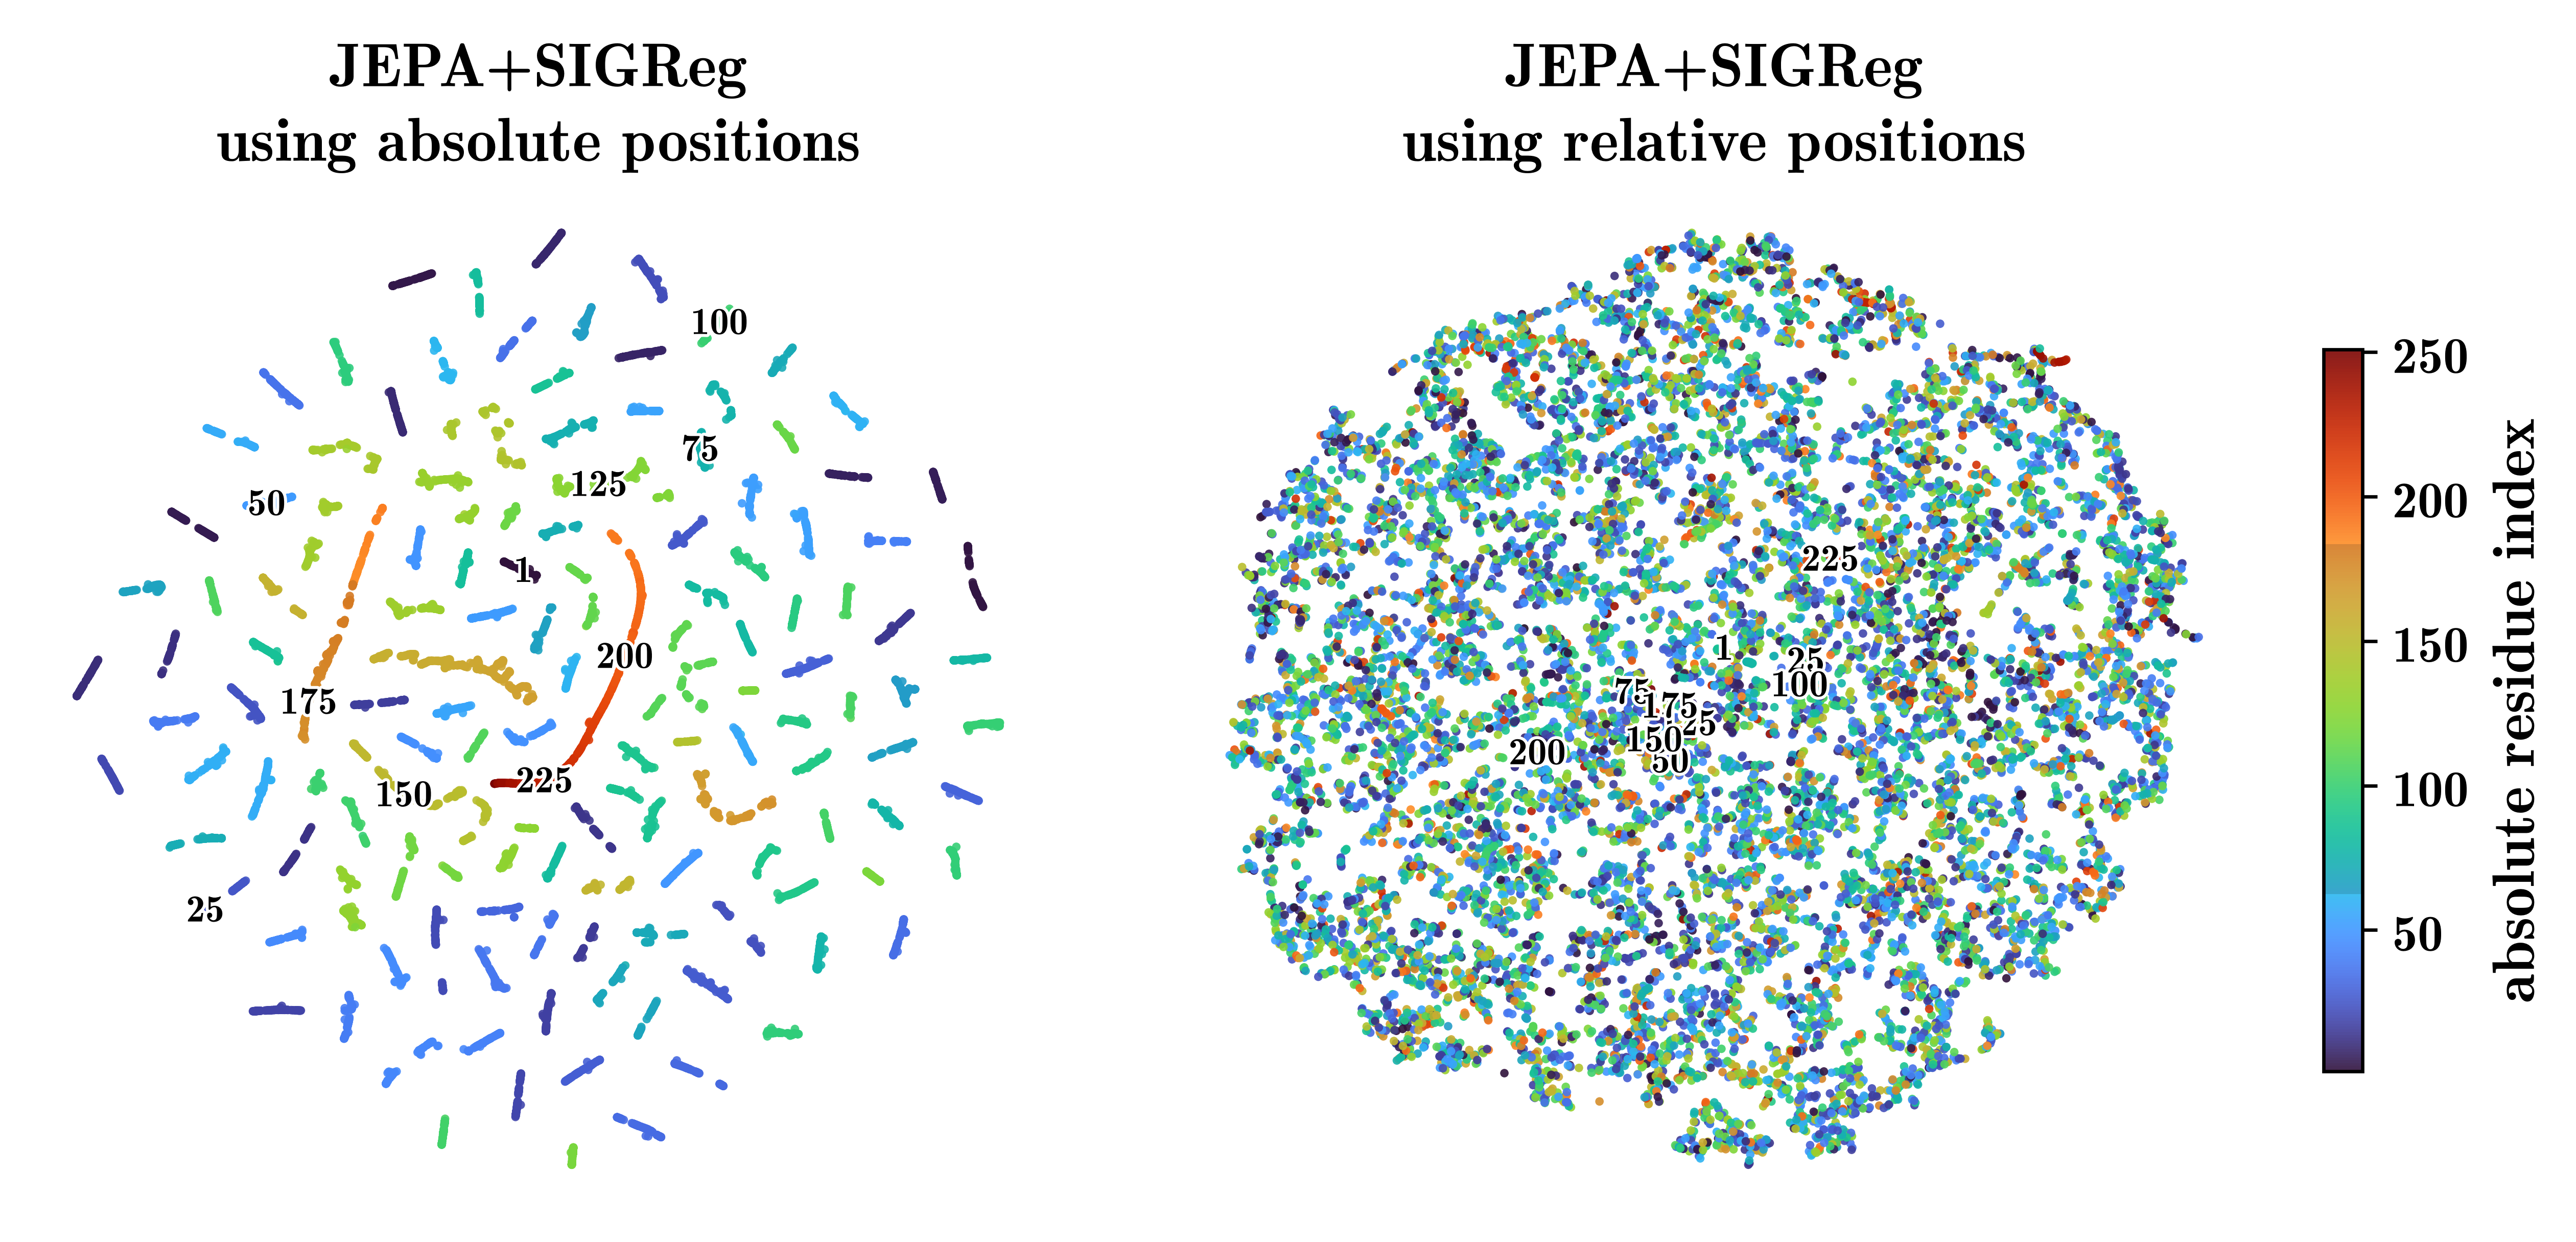
\includegraphics[width=0.90\linewidth]{tsne_jepa_sigreg_r70_absolute-v-relative_absolute-index_100k.png}
  \caption{JEPA+SIGReg with 70\% random masking at 100k steps, using absolute positions (left) and relative positions (right). Numbers and colours on the strands indicate the absolute residue index within each chain, with an index range of [1-251].}
  \label{fig:index-shortcut}
\end{figure}

Besides suppressing the residue-index shortcut, relative positioning also improves downstream performance. For 70\% masking, it increases CatBio fold AUROC ($0.529$ to $0.733$) and FlexRMSF fold correlation ($0.108$ to $0.290$), and scores higher on 19/24 task/splits. With 50\% masking, it improves on 18/24 task/splits.

\paragraph{Chain length and view design.}

Uncropped LeJEPA organises residues by chain length: residues from proteins of similar length form neighbourhoods in latent space. In the cropped version, each crop has a fixed length, regardless of the protein's chain length. To isolate the effect of cropping, we compare uncropped and cropped models while keeping every other setting unchanged, including 20\% global and 80\% local masking. Cropping reduces the chain-length correlation from $0.884$ to $0.193$, but effective rank also falls from $7.10$ to $1.61$. Retaining 80\% local masking means that only around ten visible residues remain in each 48-residue local crop, which appears too aggressive for the shorter view. We therefore use 50\% local masking in the cropped models reported in Table~\ref{tab:stb-core}, leaving around 24 visible residues and retaining near-full effective rank ($7.85/8$). The larger batch, together with the lower masking rate, likely helps maintain this healthy rank.

\begin{figure}[t]
  \centering
  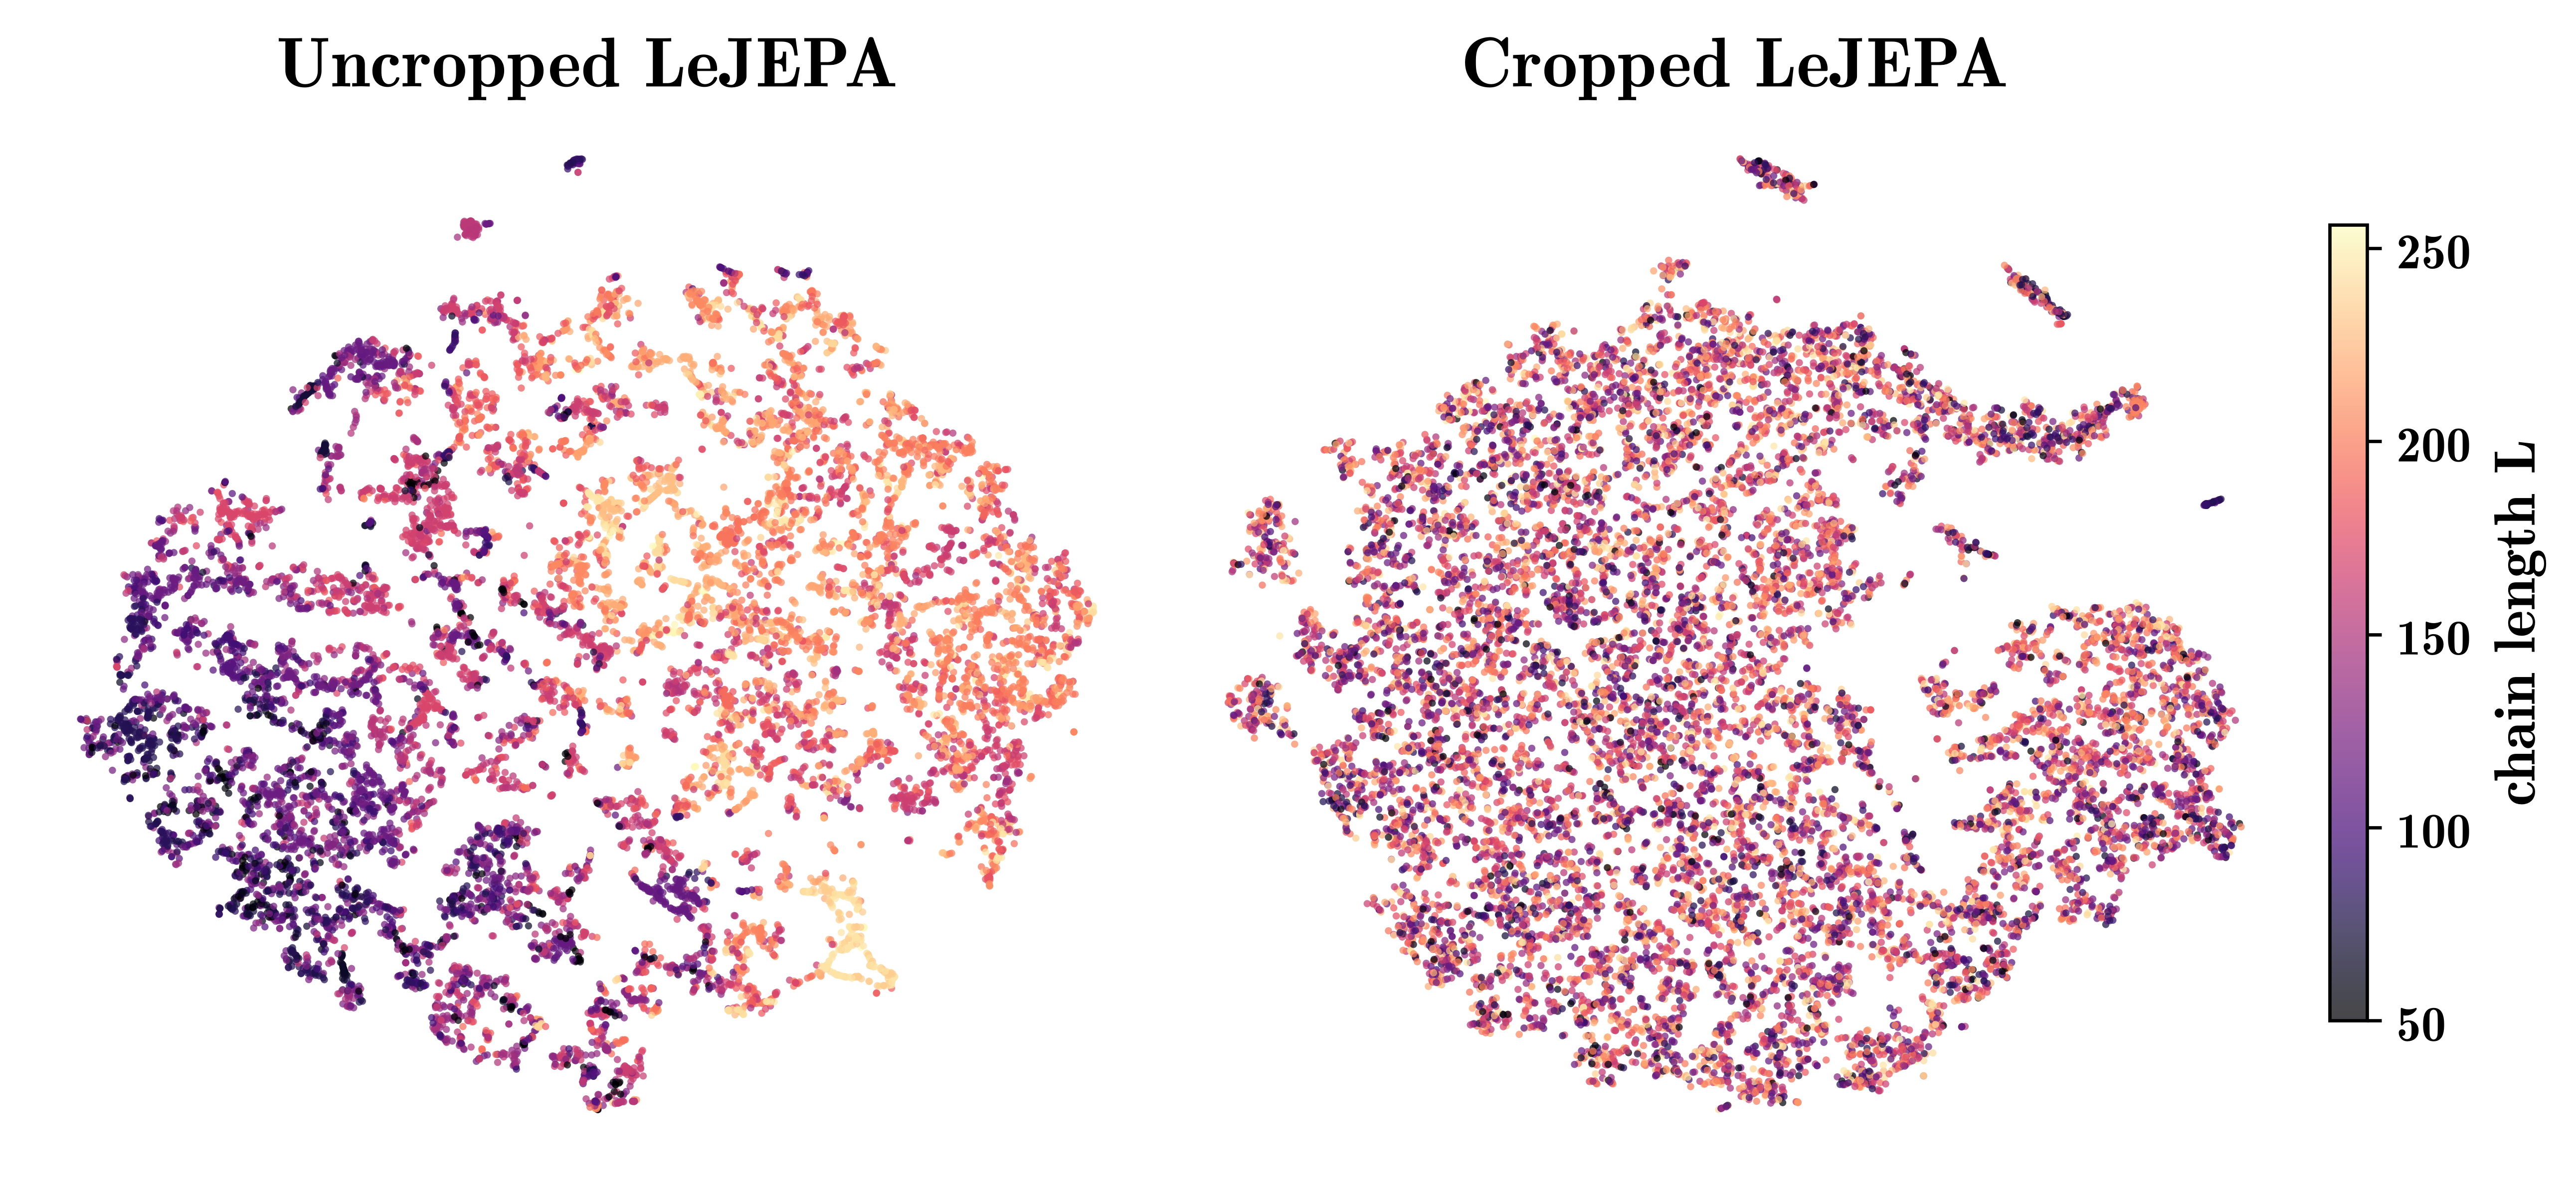
\includegraphics[width=0.88\linewidth]{chain_length_tsne_matched_crop_control_raw10k.png}
  \caption{Uncropped versus cropped LeJEPA at the 10k checkpoint. Both models use 20\% global and 80\% local masking with mean-pooled protein views. Residue embeddings are coloured by chain length. Chain-length correlation decreases from $\rho=0.884$ to $0.193$.}
  \label{fig:length-shortcut}
\end{figure}


\paragraph{Rotation invariance and effective rank.}
Beyond removing shortcuts, view design should also determine whether representations learn the intended geometric invariances. As protein properties should not depend on global orientation, we expected independent rotations to improve the learned representations more broadly. In uncropped LeJEPA at the 10k checkpoint, rotation training makes embeddings more invariant to global orientation: across 16 rotated copies of each of 400 chains, the mean cosine similarity between the same residue in different copies increases from $0.277\;[0.269,0.285]$ to $0.765\;[0.756,0.774]$ (95\% CIs) after subtracting each copy's mean embedding. The rotated model has lower effective rank ($3.22$ versus $7.17$) while scoring higher on 21/24 downstream task/splits. This suggests that learning from diverse rotated views removes orientation-dependent variation and concentrates the remaining information into fewer dimensions.

These analyses show that view construction controls both shortcut signals and geometric invariance. Suppressing a shortcut helps only when that shortcut displaces useful information. The replacement view must leave a learnable prediction problem and preserve sufficient representational variation.

\subsection{Intermediate layers expose an objective-facing bottleneck}
\label{sec:layers}

We next inspect whether information that is less accessible in the final 8D latent remains available in intermediate encoder blocks, by evaluating each block separately (Figure~\ref{fig:layerwise-stb}).

For uncropped LeJEPA, block 12 scores higher than the final 8D latent on 20/24 StructTokenBench task scores, showing that more downstream-accessible information is available before the final projection. Moving earlier in the encoder, block 4 scores higher than block 12 on 22/24 task/splits and achieves the highest score on more task/splits than any other block (9/24). Blocks 4-6 provide the highest score for 17/24 task/splits. Both block outputs are 768-dimensional, so this comparison keeps the representation width fixed. Compared with the final 8D latent, BindShake AUROC increases from $0.585$ to $0.841$, FlexRMSF fold correlation from $0.225$ to $0.654$, and all six flexibility scores are higher. Compared with a randomly initialised encoder, the trained block 6 representation scores higher on 23/24 task/splits, showing that the improvement is not explained by the 768D input alone.
The same pattern appears in JEPA with 70\% random masking: block 6 exceeds the final 8D representation on all 24 task/splits (Table~\ref{tab:jepa-r70-layerwise}, Appendix~D).

\begin{figure}[t]
  \centering
  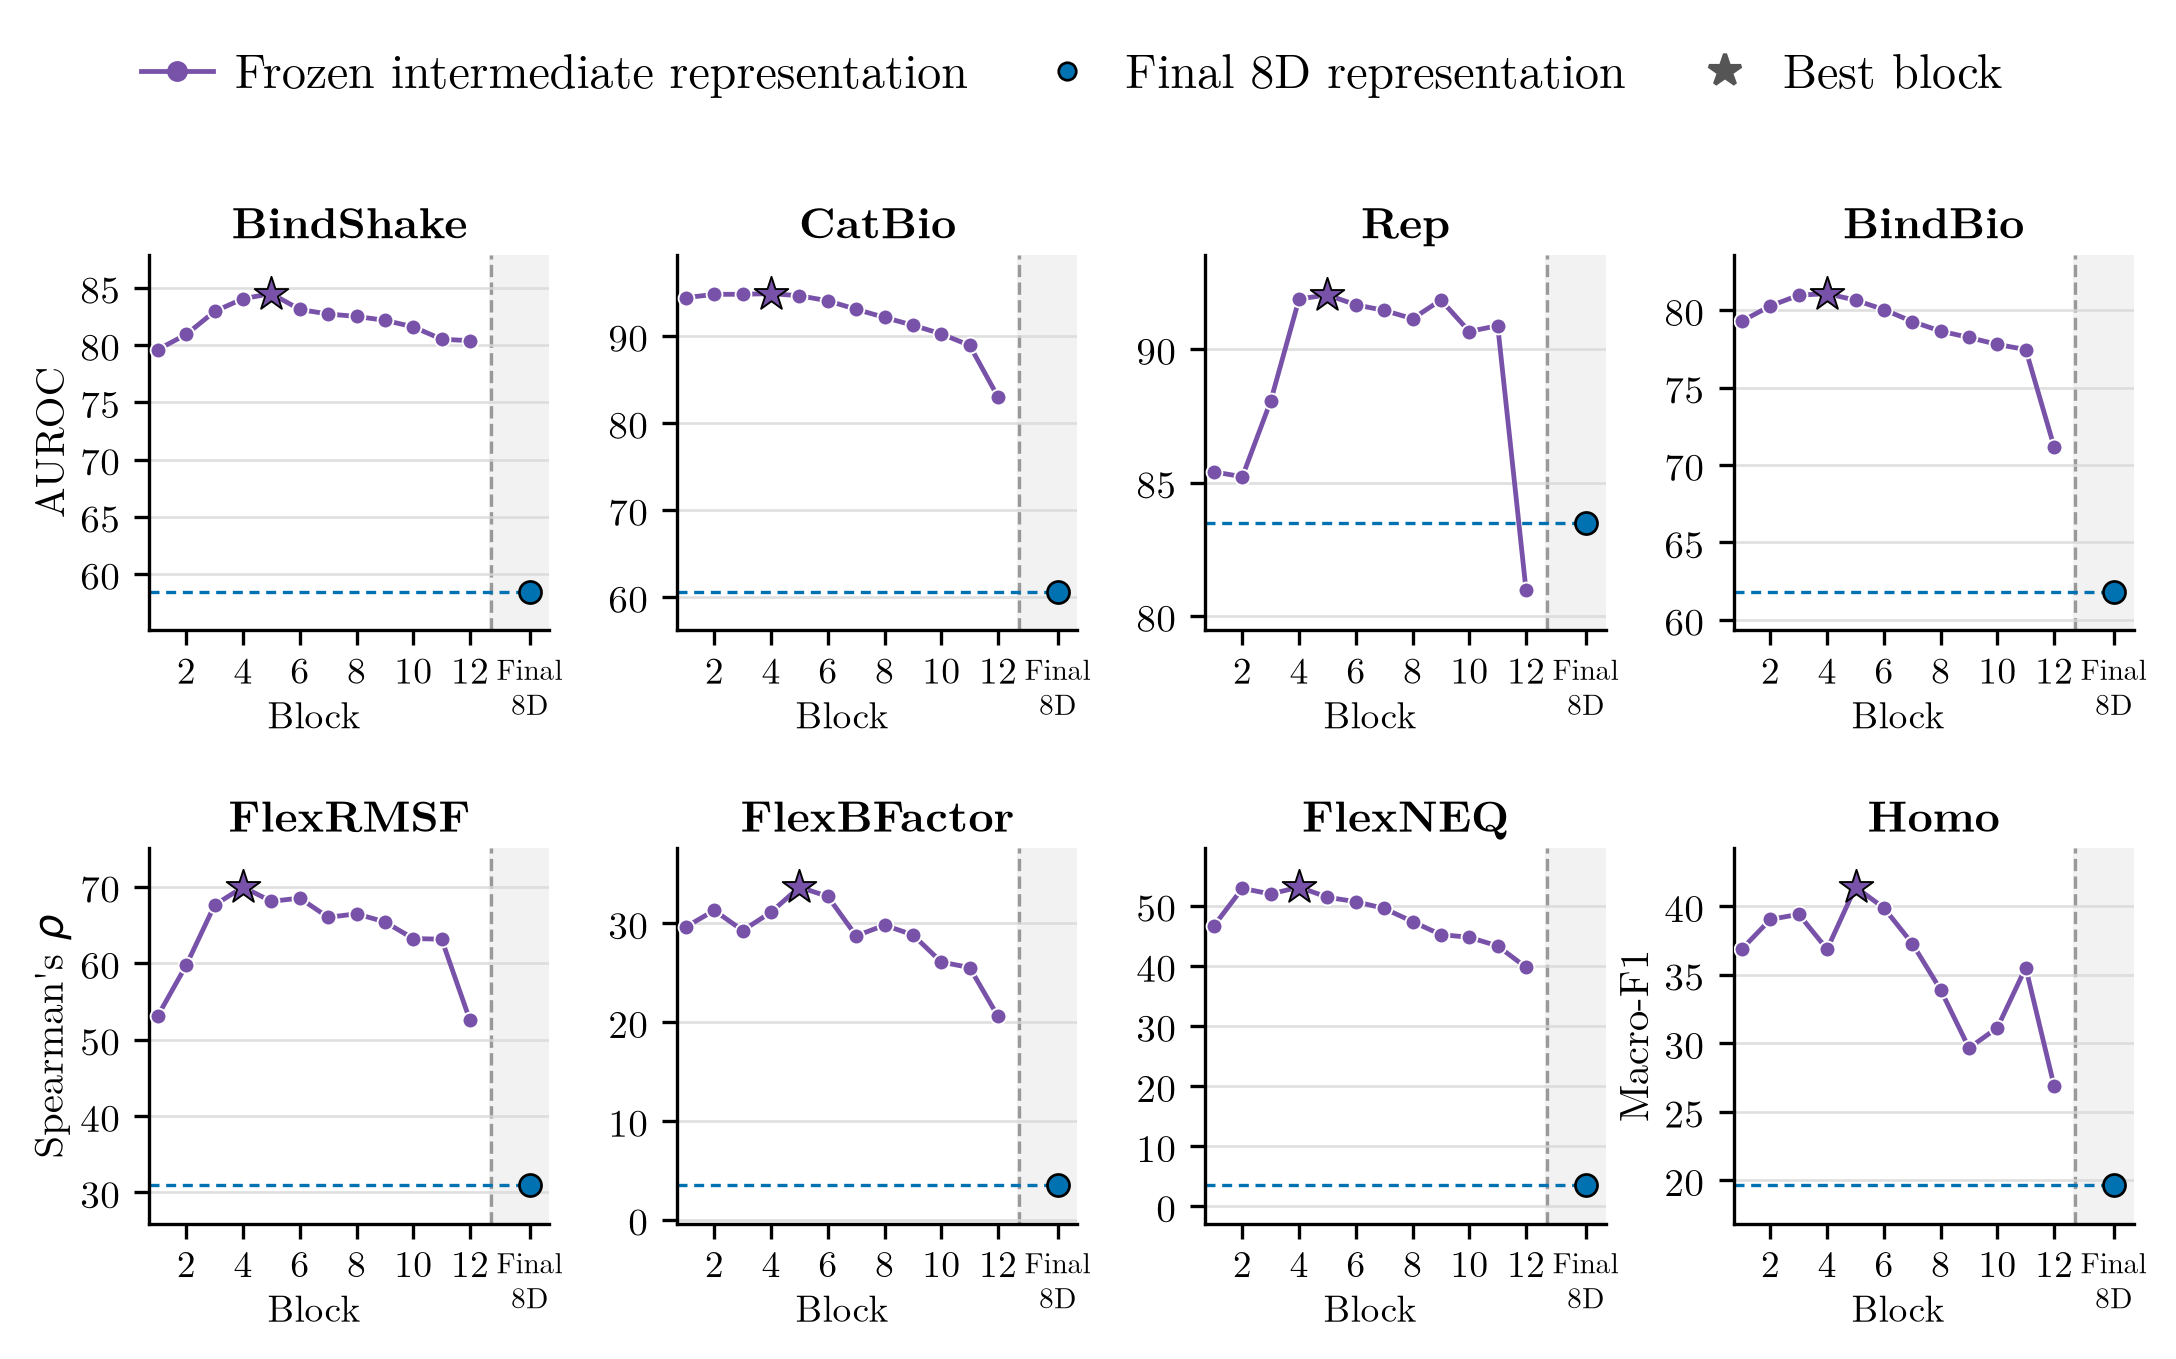
\includegraphics[width=\linewidth]{canonical_lejepa_uncropped_selected_layerwise_stb.png}
  \caption{Downstream performance across all 12 blocks of the uncropped LeJEPA encoder; scores are multiplied by 100 and stars mark the best block. The top row shows four functional-site AUROC tasks, and the bottom row shows all three structural-flexibility tasks together with remote homology. BindShake uses its original test split, Homo uses the family split, and the remaining tasks use the superfamily split. The blue point to the right of block 12 is the encoder's final 8D representation. The complete benchmark is reported in Appendix~\ref{app:layerwise-full}.}
  \label{fig:layerwise-stb}
\end{figure}

The decline from the intermediate blocks to the final 8D representation could have several causes, and we test whether two factors contribute: encoder depth and the restriction to eight dimensions.

\paragraph{Encoder depth.}
Since the intermediate blocks are most informative, we test whether a shallower encoder performs better by training uncropped LeJEPA with six encoder blocks. At 100k, its final 8D representation improves on the 12-block model's final representation on 15/24 task/splits, including all six flexibility scores. However, it remains below the 12-block encoder's intermediate block 6 on 23/24 task/splits. Thus, reducing encoder depth alone does not recover that performance. Full results are reported in Table~\ref{tab:results-encoder-depth} in Appendix~D.

\paragraph{Eight-dimensional bottleneck.}
We next ask whether an 8D representation can retain the information available in the intermediate blocks. For blocks 4, 8 and 12, we train a separate LayerNorm and linear 768D-to-8D projection jointly with each downstream task head. Across all three task families, these task-specific 8D representations remain close to their corresponding 768D block representations and outperform the encoder's final 8D representation (Figure~\ref{fig:bottleneck}, Appendix~D). Because each task learns its own projection, this does not establish that one shared 8D representation is sufficient for every task. It does show that eight dimensions can retain task-relevant information when selected for a particular task, while the shared final 8D representation does not retain the same information.

Previous work on language models similarly finds that intermediate representations can outperform final layers and explains this through the balance between preserving information and compressing it for the training objective \citep{skean2025layer}. Protein language model studies also find that the best layer depends on the downstream task, and that many tasks reuse features learned before the final layer \citep{li2024featurereuse,joeres2026taskdataset}. Our results suggest that intermediate blocks preserve information useful for downstream tasks, while later layers compress it for the pretraining objective.

\section{Discussion and Conclusion}

The central question of this paper is whether predicting or aligning latent representations can capture information useful for protein structure and function. The results support this idea, but no model is uniformly strongest. Because StructTokenBench spans residue- and protein-level properties, the task-specific results show that representations that perform well at one biological scale do not necessarily perform well at another. Enforcing orientation invariance improves most downstream scores, but not all. These differences suggest that the objective and view construction shape which information remains accessible rather than making a representation uniformly better or worse.

Masking changes both task difficulty and the shortcuts available to solve it, and harder prediction helps only when the model learns to use meaningful context. With learned absolute target positions, JEPA+SIGReg can organise its latent space almost directly by residue index. Relative offsets retain sequence separation while removing this shortcut. The reduction in index purity and improvement in downstream scores indicates that the shortcut had displaced more useful information. In LeJEPA, complete protein views expose the same chain length across views, whereas fixed-length crops reduce that organisation. Thus, a protein-specific view should remove global or local shortcuts without making the remaining prediction problem uninformative or excessively difficult.

JEPA pretraining produces biologically informative internal protein representations, but the objective's projection can discard information useful for downstream tasks. The layerwise results show that useful information can remain accessible inside the encoder even when it is not retained in the final latent. Downstream evaluation should therefore include intermediate encoder representations.

Future work should repeat the central experiments across seeds and extend the mask and crop sweeps. It should test different model depths and latent widths, longer training, and initialisation from pretrained La-Proteina. Evaluation beyond StructTokenBench, particularly on ATOM3D and TAPE \citep{townshend2020atom3d,rao2019tape}, would test whether the results generalise. Finally, intermediate layers could be used for early-exit prediction \citep{hart2026protein}, while refining pretraining objectives could help preserve transferable information in the final representation.

This paper adapts JEPA and LeJEPA objectives to residue-level all-atom protein structures and develops a framework for examining what their representations learn. The experiments show that predictive learning can support both downstream transfer and detailed latent-space analysis, while exposing shortcuts based on residue position and chain length. Together, these findings provide practical guidance for future all-atom protein JEPAs: construct protein-appropriate views, test representations for shortcut signals, and evaluate information throughout the encoder rather than only at its final output.

\subsection*{AI use statement}
Generative AI assisted iterative wording, code and figure preparation, and feedback on experimental design. The research ideas and experiments are our own. We reviewed all AI-assisted material and take responsibility for the final content.

\subsection*{Reproducibility statement}
Section~\ref{sec:method} and Appendix~\ref{app:training} describe the data, models, objectives, evaluation and training settings. Complete results and supporting experiments are provided in the remaining appendices.

\bibliography{references}
\bibliographystyle{iclr2027_conference}

\clearpage
\appendix

\section{Complete StructTokenBench Results}
\begin{table}[!ht]
\centering
\setlength{\tabcolsep}{1.65pt}
\renewcommand{\arraystretch}{0.97}
\fontsize{7.8}{9.6}\selectfont
\caption{Complete StructTokenBench results for the 18 evaluated 100k configurations. Models are rows and tasks and holdout splits are columns. Scores are multiplied by 100 and higher is better.}
\label{tab:stb-all-100k}

\resizebox{\linewidth}{!}{%
\begin{tabular}{@{}l*{4}{r}c*{10}{r}@{}}
\toprule
 & \multicolumn{15}{c}{Functional-site prediction: AUROC $\times100$} \\
Model & \multicolumn{2}{c}{BindInt} & \multicolumn{2}{c}{BindBio} & BindShake & \multicolumn{2}{c}{CatInt} & \multicolumn{2}{c}{CatBio} & \multicolumn{2}{c}{Con} & \multicolumn{2}{c}{Rep} & \multicolumn{2}{c}{Ept} \\
\cmidrule(lr){2-3}\cmidrule(lr){4-5}\cmidrule(lr){6-6}\cmidrule(lr){7-8}\cmidrule(lr){9-10}\cmidrule(lr){11-12}\cmidrule(lr){13-14}\cmidrule(lr){15-16}
 & Fold & SF & Fold & SF & Org. & Fold & SF & Fold & SF & Fold & SF & Fold & SF & Fold & SF \\
\midrule
\multicolumn{16}{@{}l}{\textbf{Autoencoders}} \\
$C_\alpha$ AE (EMA) & 44.60 & 80.01 & 63.12 & 63.77 & 59.21 & 54.53 & 77.70 & 67.22 & 73.66 & 56.53 & 70.58 & 75.12 & 79.58 & 47.08 & 53.60 \\
Fully latent AE (EMA) & 44.82 & 81.48 & 69.61 & 69.65 & 76.06 & 59.86 & 80.08 & 77.30 & 83.56 & 61.62 & 74.96 & 73.60 & 80.44 & 47.74 & 52.38 \\
\midrule
\multicolumn{16}{@{}l}{\textbf{JEPA}} \\
Rand 50\% & 44.46 & 81.67 & 60.59 & 61.80 & 62.32 & 56.86 & 72.55 & 59.31 & 65.61 & 57.55 & 71.05 & 75.12 & 81.34 & 46.92 & 49.75 \\
Rand 70\% & 47.11 & 80.06 & 65.56 & 65.31 & 71.85 & 56.84 & 76.71 & 71.50 & 75.36 & 60.44 & 72.08 & 73.77 & 78.46 & 47.87 & 49.29 \\
Mutation & 45.46 & 81.84 & 63.96 & 64.56 & 68.75 & 56.68 & 77.13 & 68.03 & 72.36 & 60.33 & 72.10 & 73.55 & 79.92 & 51.38 & 53.11 \\
\midrule
\multicolumn{16}{@{}l}{\textbf{JEPA+SIGReg}} \\
Rand 50\% (abs. pos.) & 45.32 & 82.51 & 58.82 & 60.82 & 59.73 & 55.36 & 76.86 & 52.75 & 58.09 & 58.05 & 72.96 & 75.93 & 81.37 & 53.67 & 56.80 \\
Rand 70\% (abs. pos.) & 43.13 & 82.54 & 59.02 & 61.05 & 59.72 & 54.49 & 77.38 & 52.92 & 58.43 & 58.49 & 73.08 & 75.65 & 80.58 & 53.99 & 55.83 \\
Mutation & 43.97 & 83.01 & 58.57 & 60.60 & 59.82 & 55.81 & 77.48 & 52.85 & 58.14 & 57.54 & 72.51 & 75.14 & 80.75 & 51.80 & 53.99 \\
Rand 50\% (rel. pos.) & 46.43 & 81.26 & 66.98 & 67.20 & 74.66 & 62.28 & 79.76 & 74.04 & 78.70 & 60.68 & 74.25 & 75.17 & 79.68 & 51.75 & 58.90 \\
Rand 70\% (rel. pos.) & 47.39 & 82.62 & 66.09 & 66.25 & 73.05 & 60.24 & 79.81 & 73.28 & 78.20 & 62.35 & 74.12 & 74.48 & 81.18 & 52.43 & 56.61 \\
Chem: 50\% atoms & 45.24 & 78.97 & 59.11 & 59.94 & 62.84 & 54.03 & 76.44 & 60.61 & 65.97 & 56.62 & 70.10 & 74.89 & 78.25 & 52.51 & 53.21 \\
Chem: no AA+50\% SC & 45.54 & 80.10 & 65.15 & 65.08 & 70.85 & 57.76 & 74.59 & 72.62 & 76.39 & 58.18 & 71.76 & 74.54 & 78.62 & 55.99 & 59.98 \\
Spatial (rel. pos.) & 49.46 & 82.85 & 65.56 & 65.96 & 71.87 & 63.10 & 80.96 & 71.60 & 76.70 & 62.16 & 76.23 & 74.11 & 79.92 & 51.55 & 59.31 \\
Rand 70\% (rel. pos.)+SO(3) & 48.79 & 89.37 & 65.01 & 65.38 & 68.55 & 63.18 & 84.28 & 67.25 & 73.30 & 56.04 & 78.28 & 72.98 & 85.63 & 53.52 & 57.93 \\
\midrule
\multicolumn{16}{@{}l}{\textbf{LeJEPA}} \\
Uncropped & 50.30 & 88.45 & 59.32 & 61.82 & 58.45 & 51.71 & 80.74 & 53.67 & 60.61 & 60.10 & 77.27 & 71.05 & 83.49 & 62.00 & 59.72 \\
Uncropped (EMA) & 49.87 & 88.49 & 59.31 & 61.73 & 58.24 & 53.43 & 80.50 & 53.68 & 60.52 & 60.30 & 77.32 & 72.85 & 84.43 & 63.05 & 61.62 \\
Uncropped+SO(3) & 46.27 & 91.65 & 59.72 & 62.66 & 61.24 & 59.94 & 83.53 & 53.21 & 62.57 & 55.79 & 83.10 & 71.50 & 82.87 & 53.14 & 60.30 \\
Uncropped+SO(3) (EMA) & 45.36 & 91.71 & 59.69 & 62.93 & 60.80 & 56.07 & 83.77 & 53.95 & 62.68 & 56.07 & 83.06 & 68.95 & 85.14 & 54.35 & 59.25 \\
\bottomrule
\end{tabular}%
}

\medskip
\begin{tabular}{@{}l@{\hspace{6pt}}*{3}{r}@{\hspace{5pt}}*{6}{r}@{}}
\toprule
 & \multicolumn{3}{c}{Homo: macro-F1 $\times100$} & \multicolumn{6}{c}{Flexibility: Spearman's $\rho\times100$} \\
Model & Fold & Fam. & SF & \multicolumn{2}{c}{FlexRMSF} & \multicolumn{2}{c}{FlexBFactor} & \multicolumn{2}{c}{FlexNEQ} \\
\cmidrule(lr){5-6}\cmidrule(lr){7-8}\cmidrule(lr){9-10}
 & & & & Fold & SF & Fold & SF & Fold & SF \\
\midrule
\multicolumn{10}{@{}l}{\textbf{Autoencoders}} \\
$C_\alpha$ AE (EMA) & 6.67 & 20.15 & 4.23 & 16.01 & 12.15 & 11.32 & 10.75 & 14.35 & 12.65 \\
Fully latent AE (EMA) & 8.23 & 14.36 & 5.13 & 42.83 & 41.04 & 28.81 & 24.27 & 20.13 & 19.57 \\
\midrule
\multicolumn{10}{@{}l}{\textbf{JEPA}} \\
Rand 50\% & 7.79 & 16.67 & 4.18 & 29.45 & 34.39 & 12.90 & 12.20 & 9.10 & 12.43 \\
Rand 70\% & 9.86 & 13.30 & 6.00 & 33.98 & 34.26 & 23.29 & 21.69 & 25.11 & 25.19 \\
Mutation & 8.01 & 11.82 & 4.61 & 35.08 & 35.61 & 22.09 & 17.76 & 10.07 & 10.60 \\
\midrule
\multicolumn{10}{@{}l}{\textbf{JEPA+SIGReg}} \\
Rand 50\% (abs. pos.) & 6.94 & 13.23 & 3.23 & 6.95 & 3.21 & 3.67 & 2.10 & 3.58 & 5.41 \\
Rand 70\% (abs. pos.) & 8.03 & 13.60 & 4.06 & 10.83 & 2.16 & 3.28 & 1.75 & 4.47 & 3.92 \\
Mutation & 6.44 & 12.88 & 3.41 & 9.84 & 3.22 & 4.53 & 2.34 & 4.65 & 3.04 \\
Rand 50\% (rel. pos.) & 6.26 & 12.10 & 3.65 & 31.56 & 25.92 & 21.04 & 19.42 & 16.82 & 14.08 \\
Rand 70\% (rel. pos.) & 6.67 & 11.06 & 3.64 & 28.97 & 24.78 & 19.82 & 18.23 & 15.10 & 11.36 \\
Chem: 50\% atoms & 8.41 & 18.24 & 4.24 & 14.57 & 12.33 & 5.25 & 6.17 & 8.73 & 9.99 \\
Chem: no AA+50\% SC & 7.24 & 12.15 & 4.04 & 27.65 & 22.49 & 17.42 & 17.38 & 16.58 & 17.41 \\
Spatial (rel. pos.) & 8.62 & 11.95 & 4.81 & 27.99 & 24.92 & 18.55 & 17.04 & 12.22 & 10.48 \\
Rand 70\% (rel. pos.)+SO(3) & 6.71 & 16.01 & 4.36 & 18.45 & 15.34 & 12.46 & 12.32 & 12.08 & 12.22 \\
\midrule
\multicolumn{10}{@{}l}{\textbf{LeJEPA}} \\
Uncropped & 6.73 & 19.64 & 5.54 & 22.48 & 30.96 & 5.01 & 3.50 & 2.46 & 3.54 \\
Uncropped (EMA) & 7.59 & 21.70 & 5.40 & 22.62 & 33.21 & 3.14 & 7.72 & 7.86 & 6.15 \\
Uncropped+SO(3) & 9.96 & 27.60 & 12.67 & 35.51 & 43.51 & 22.44 & 18.08 & 6.56 & 7.37 \\
Uncropped+SO(3) (EMA) & 11.68 & 33.63 & 12.90 & 35.15 & 42.82 & 22.18 & 19.27 & 5.98 & 7.42 \\
\bottomrule
\end{tabular}

\par\smallskip
\fontsize{7.2}{8.4}\selectfont
Fam. = family; SF = superfamily; Org. = original benchmark split. Homo is the mean of batch-level macro-F1. AA denotes amino-acid identity and SC denotes side-chain coordinates.
\end{table}
\clearpage

The complete table includes additional masking ablations that are not part of the main comparison. Spatial masking selects separated C$\alpha$ seed residues and masks local neighbourhoods extending up to a 30\,\AA{} radius, hiding approximately 75\% of the protein. Chemical masks retain partial information at target positions: coordinate masking retains amino-acid identity and hides 50\% of observed atom coordinates, while side-chain masking hides amino-acid identity and 50\% of observed side-chain coordinates but retains the backbone.

\begin{table}[!ht]
\centering
\setlength{\tabcolsep}{1.65pt}
\renewcommand{\arraystretch}{0.97}
\fontsize{7.8}{9.6}\selectfont
\caption{Complete StructTokenBench results for the four cropped LeJEPA configurations at raw 10k checkpoints. Models are rows and tasks and holdout splits are columns. Scores are multiplied by 100 and higher is better. These runs use batch size 96 and are not compute-matched to the 100k configurations.}
\label{tab:stb-all-crops}

\resizebox{\linewidth}{!}{%
\begin{tabular}{@{}l*{4}{r}c*{10}{r}@{}}
\toprule
 & \multicolumn{15}{c}{Functional-site prediction: AUROC $\times100$} \\
Model & \multicolumn{2}{c}{BindInt} & \multicolumn{2}{c}{BindBio} & BindShake & \multicolumn{2}{c}{CatInt} & \multicolumn{2}{c}{CatBio} & \multicolumn{2}{c}{Con} & \multicolumn{2}{c}{Rep} & \multicolumn{2}{c}{Ept} \\
\cmidrule(lr){2-3}\cmidrule(lr){4-5}\cmidrule(lr){6-6}\cmidrule(lr){7-8}\cmidrule(lr){9-10}\cmidrule(lr){11-12}\cmidrule(lr){13-14}\cmidrule(lr){15-16}
 & Fold & SF & Fold & SF & Org. & Fold & SF & Fold & SF & Fold & SF & Fold & SF & Fold & SF \\
\midrule
Per protein & 48.32 & 86.59 & 57.66 & 58.95 & 58.81 & 56.47 & 81.00 & 56.67 & 62.18 & 55.04 & 73.63 & 74.30 & 81.89 & 47.04 & 58.22 \\
Per protein+SO(3) & 53.11 & 89.54 & 60.79 & 63.73 & 61.77 & 53.33 & 83.94 & 65.06 & 70.55 & 56.07 & 77.51 & 74.78 & 87.43 & 56.42 & 55.24 \\
Per residue & 44.14 & 82.87 & 57.85 & 59.03 & 60.67 & 55.28 & 77.44 & 57.82 & 61.57 & 55.67 & 71.23 & 74.41 & 79.69 & 50.56 & 52.64 \\
Per residue+SO(3) & 48.06 & 89.59 & 65.28 & 67.27 & 66.65 & 55.63 & 84.13 & 70.78 & 71.26 & 57.00 & 76.32 & 73.34 & 83.82 & 50.65 & 54.79 \\
\bottomrule
\end{tabular}%
}

\medskip
\begin{tabular}{@{}l@{\hspace{7pt}}*{3}{r}@{\hspace{7pt}}*{6}{r}@{}}
\toprule
 & \multicolumn{3}{c}{Homo: macro-F1 $\times100$} & \multicolumn{6}{c}{Flexibility: Spearman's $\rho\times100$} \\
Model & Fold & Fam. & SF & \multicolumn{2}{c}{FlexRMSF} & \multicolumn{2}{c}{FlexBFactor} & \multicolumn{2}{c}{FlexNEQ} \\
\cmidrule(lr){5-6}\cmidrule(lr){7-8}\cmidrule(lr){9-10}
 & & & & Fold & SF & Fold & SF & Fold & SF \\
\midrule
Per protein & 19.36 & 29.30 & 13.51 & 19.01 & 25.46 & 9.73 & 10.18 & 20.00 & 19.16 \\
Per protein+SO(3) & 27.72 & 58.03 & 28.64 & 29.77 & 30.13 & 16.07 & 14.77 & 21.75 & 21.40 \\
Per residue & 9.44 & 17.32 & 5.55 & 16.55 & 16.06 & 9.58 & 10.07 & 49.33 & 49.72 \\
Per residue+SO(3) & 21.96 & 30.07 & 11.83 & 36.06 & 30.70 & 18.41 & 16.88 & 59.37 & 58.58 \\
\bottomrule
\end{tabular}

\par\smallskip
\fontsize{7.2}{8.4}\selectfont
Fam. = family; SF = superfamily; Org. = original benchmark split. Homo is the mean of batch-level macro-F1.
\end{table}

\clearpage

\section{JEPA Architectures}

\begin{figure}[!h]
  \centering
  \includegraphics[width=0.72\linewidth]{JEPA.pdf}
  \caption{JEPA architecture, illustrated with 50\% random masking. The context encoder processes visible residues, the EMA target encoder processes the complete protein, and the cross-attention predictor predicts the selected target-residue latents.}
  \label{fig:jepa-architecture}
\end{figure}

\begin{figure}[!h]
  \centering
  \includegraphics[width=0.72\linewidth]{JEPA_SIGReg.pdf}
  \caption{JEPA+SIGReg architecture. A shared encoder processes the masked context and complete target views, while a cross-attention predictor predicts the selected target-residue latents. Training combines the prediction loss with SIGReg.}
  \label{fig:jepa-sigreg-architecture}
\end{figure}
\clearpage

\section{Training Settings and Reproducibility}
\label{app:training}

JEPA and JEPA+SIGReg use a batch size of 4, a peak learning rate of $10^{-4}$ that is reduced when validation performance plateaus, and weight decay of $10^{-2}$. Following LeVJEPA, LeJEPA uses a peak learning rate of $4\times10^{-4}$ with linear warmup and weight decay of $0.04$. Uncropped LeJEPA uses a batch size of 16, while cropped LeJEPA uses a batch size of 96. All models use AdamW and seed 42.

The main results use 100,000-step checkpoints, except cropped LeJEPA, which uses 10,000-step checkpoints. Its larger batch gives a similar order of protein presentations despite the shorter training. Due to memory and compute constraints, the reported configurations are single training runs.

\section{Supporting Experiments}

\subsection{Separately trained six-block encoder}
\label{app:encoder-depth}

Table~\ref{tab:results-encoder-depth} compares the final 8D representations of separately trained six- and twelve-block uncropped LeJEPA encoders with the intermediate block 6 representation of the twelve-block encoder. Both full models use seed 42, and the StructTokenBench cohorts and downstream predictor configurations match. Each depth was trained once, so the differences have not been checked across independent training seeds.

\begin{table}[!htbp]
\centering
\setlength{\tabcolsep}{4pt}
\renewcommand{\arraystretch}{0.86}
\fontsize{7.6}{8.8}\selectfont
\caption{StructTokenBench comparison of uncropped LeJEPA with 12 and 6 encoder blocks, without rotations, using weights at 100k. Scores are multiplied by 100. Bold marks the highest score in each row. The first two model columns use the final 8D representation, the third uses the intermediate 768D representation from block 6 of the 12-block encoder, and the fourth is the corresponding block from a randomly initialised encoder.}
\label{tab:results-encoder-depth}
\begin{tabular}{@{}llrrrr@{}}
\toprule
Task & Split & \shortstack{12-block model\\Final 8D} & \shortstack{6-block model\\Final 8D} & \shortstack{12-block model\\Block 6, 768D} & \shortstack{Random init.\\Block 6, 768D} \\
\midrule
\multicolumn{6}{c}{\textbf{Functional-site prediction: AUROC $\times100$}} \\
\midrule
BindInt & Fold & 50.30 & 45.81 & \textbf{52.19} & 48.98 \\
 & SF & 88.45 & 88.58 & \textbf{94.13} & 88.06 \\
BindBio & Fold & 59.32 & 59.28 & \textbf{78.31} & 74.12 \\
 & SF & 61.82 & 61.41 & \textbf{80.04} & 74.58 \\
BindShake & Test & 58.45 & 59.15 & \textbf{83.11} & 78.23 \\
CatInt & Fold & 51.71 & 57.13 & \textbf{69.36} & 64.32 \\
 & SF & 80.74 & 79.20 & \textbf{95.78} & 88.95 \\
CatBio & Fold & 53.67 & 54.06 & \textbf{85.05} & 81.87 \\
 & SF & 60.61 & 60.50 & \textbf{94.04} & 91.41 \\
Con & Fold & 60.10 & 58.07 & \textbf{68.22} & 63.47 \\
 & SF & 77.27 & 78.01 & \textbf{92.16} & 81.40 \\
Rep & Fold & 71.05 & 73.05 & 60.39 & \textbf{76.66} \\
 & SF & 83.49 & 83.64 & \textbf{91.66} & 79.48 \\
Ept & Fold & \textbf{62.00} & 54.51 & 55.70 & 55.61 \\
 & SF & 59.72 & 58.83 & \textbf{76.09} & 69.06 \\
\midrule
\multicolumn{6}{c}{\textbf{Remote homology: macro-F1 $\times100$}} \\
\midrule
Homo & Fold & 6.73 & 7.73 & \textbf{16.94} & 6.64 \\
 & Family & 19.64 & 16.70 & \textbf{39.88} & 21.76 \\
 & SF & 5.54 & 6.56 & \textbf{19.90} & 6.77 \\
\midrule
\multicolumn{6}{c}{\textbf{Structural flexibility: Spearman's $\rho\times100$}} \\
\midrule
FlexRMSF & Fold & 22.48 & 29.84 & \textbf{63.39} & 43.84 \\
 & SF & 30.96 & 41.25 & \textbf{68.52} & 41.73 \\
FlexBFactor & Fold & 5.01 & 6.54 & \textbf{37.71} & 31.14 \\
 & SF & 3.50 & 5.11 & \textbf{32.73} & 27.15 \\
FlexNEQ & Fold & 2.46 & 4.19 & \textbf{51.39} & 19.11 \\
 & SF & 3.54 & 5.21 & \textbf{50.69} & 19.29 \\
\bottomrule
\end{tabular}
\end{table}
\clearpage

\subsection{Complete layerwise StructTokenBench evaluation}
\label{app:layerwise-full}

\begin{figure}[!htbp]
  \centering
  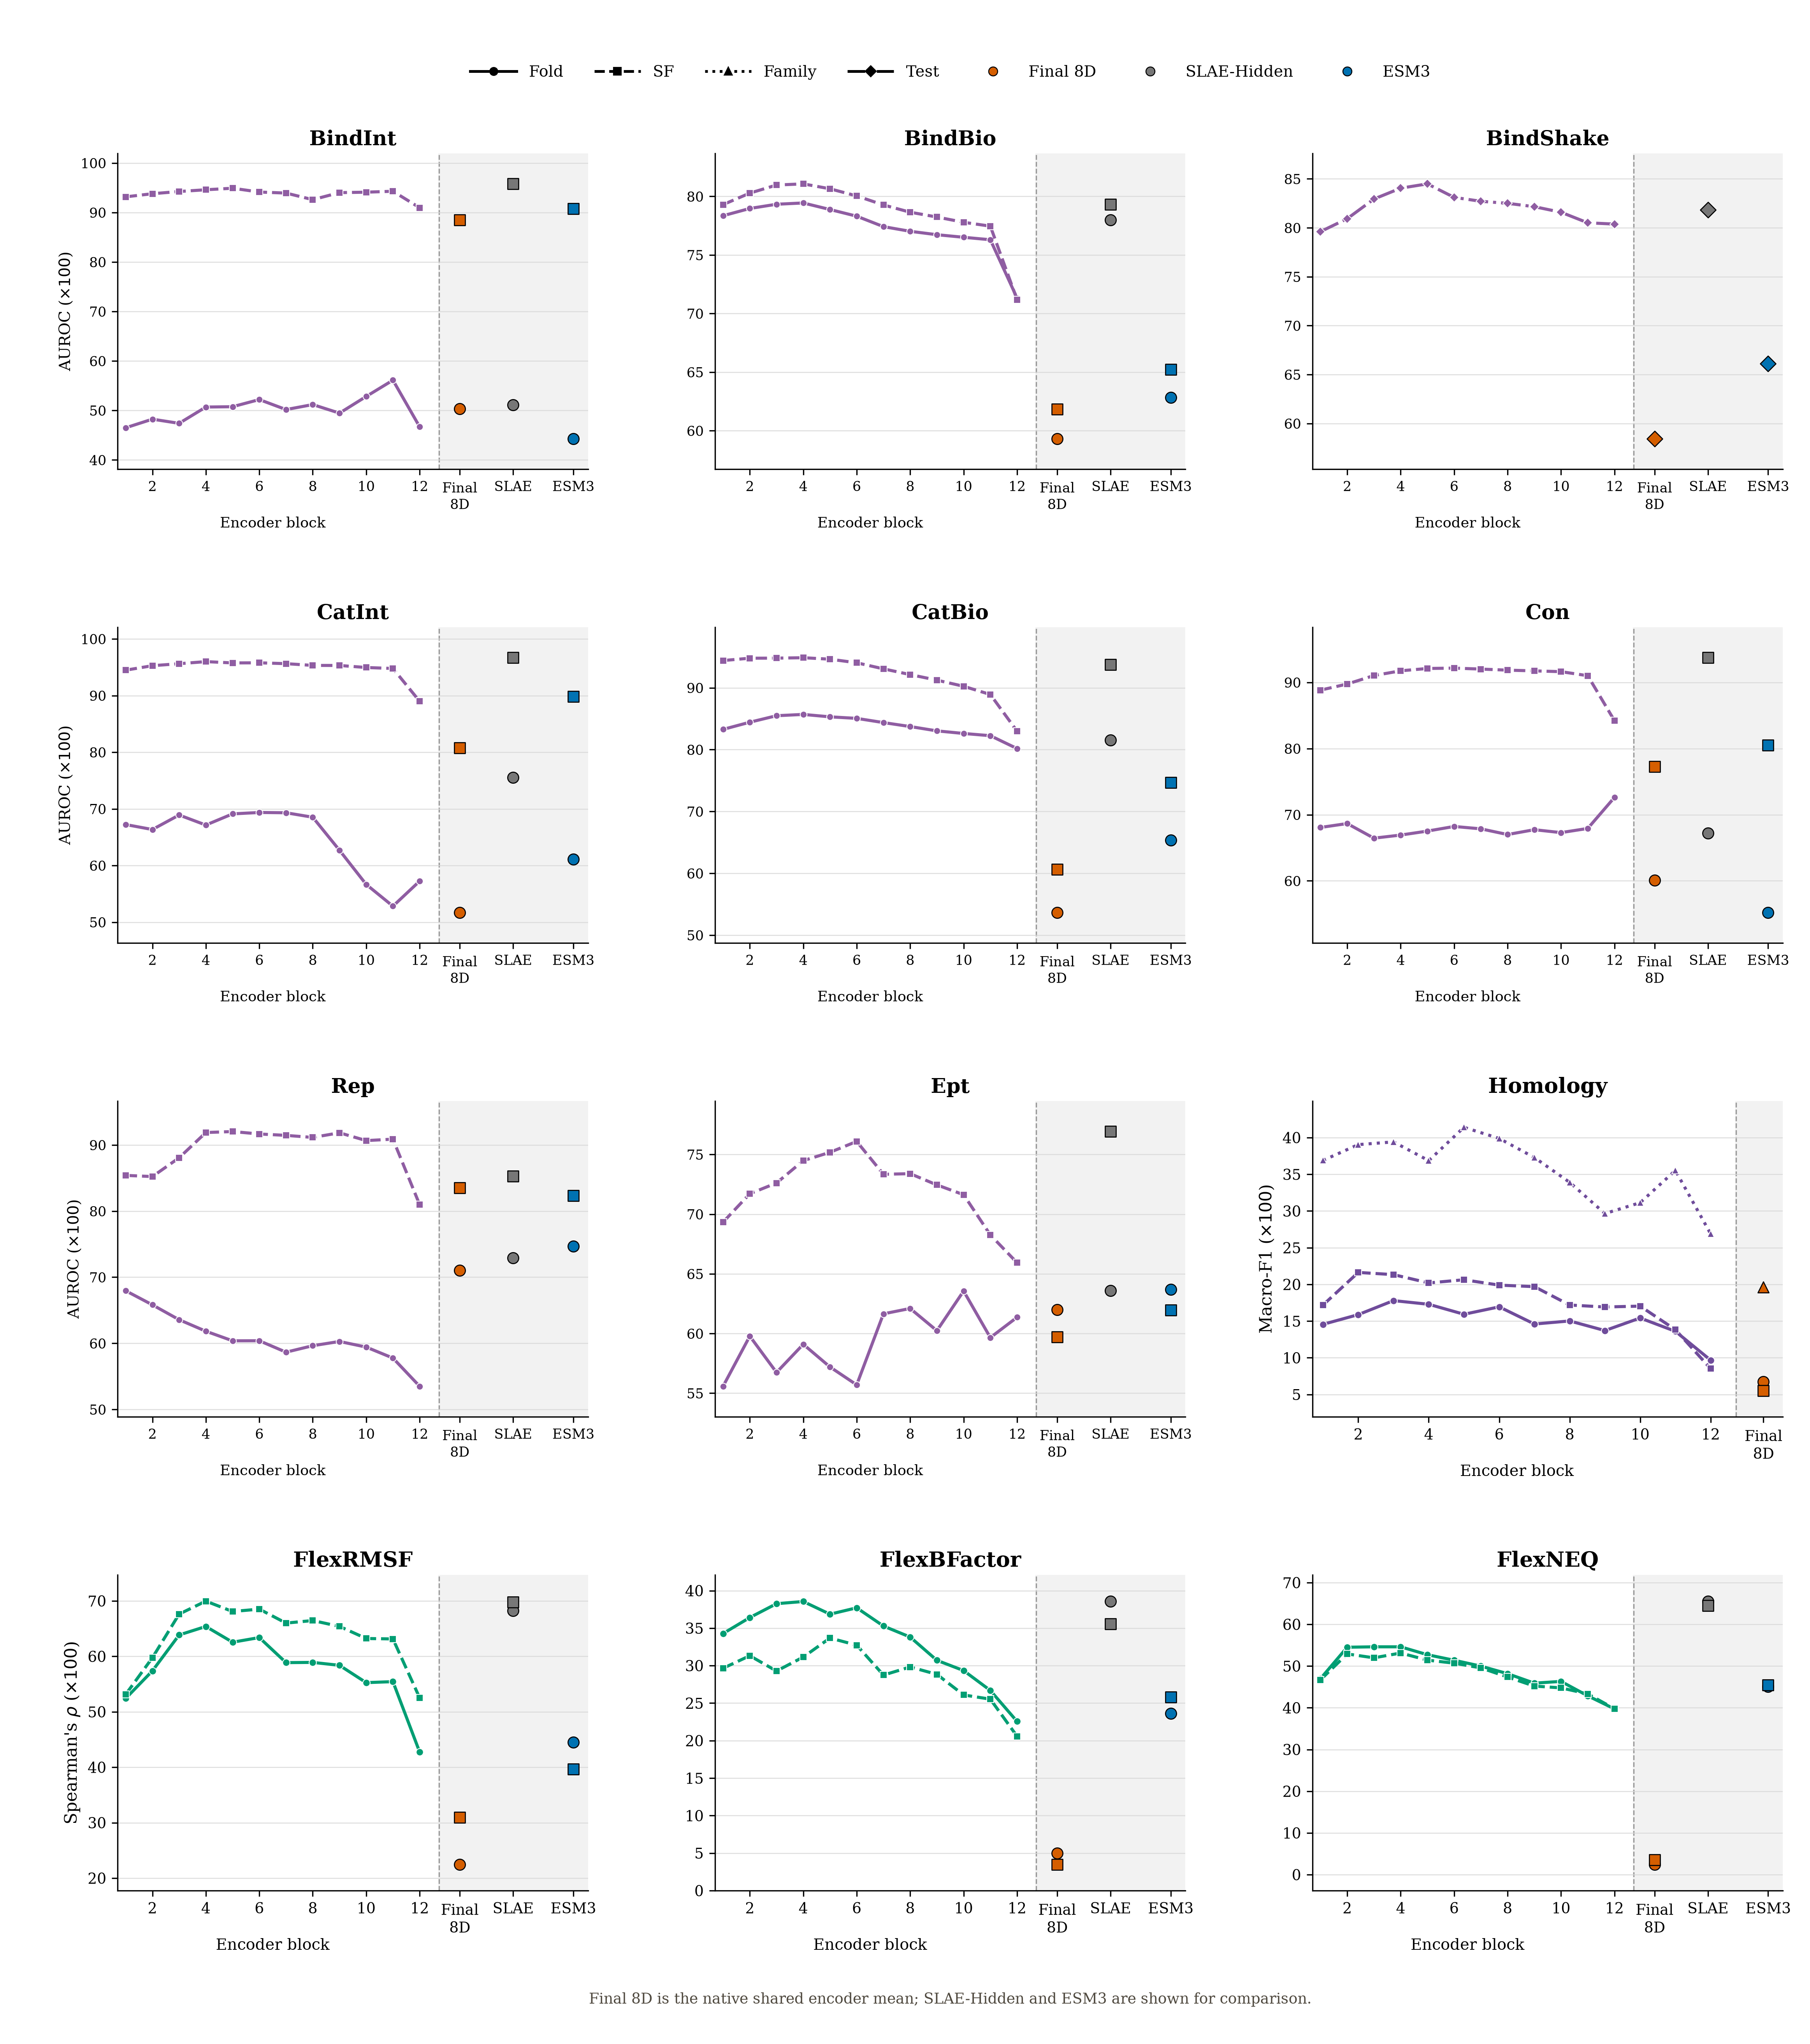
\includegraphics[width=\linewidth,height=0.89\textheight,keepaspectratio]{canonical_lejepa_raw100k_layerwise_stb_all_metrics.png}
  \caption{Complete layerwise StructTokenBench evaluation for uncropped LeJEPA without rotations at 100k steps, using online weights and full-context evaluation. Blocks expose frozen 768D post-block representations. Final 8D is the encoder's final representation. SLAE-Hidden and ESM3 results are taken from the SLAE paper \citep{chen2026slae} and included only where the task, split and metric definitions match.}
  \label{fig:layerwise-stb-full}
\end{figure}
\clearpage

\subsection{Task-supervised 8D bottlenecks}

For blocks 4, 8 and 12, we keep the encoder frozen and train a separate $\operatorname{LayerNorm}(768)\rightarrow\operatorname{Linear}(768,8)$ projection jointly with each StructTokenBench task head. The projection is therefore supervised by one downstream task and is not a shared pretrained latent. All nine block-by-task-family averages exceed the encoder's final 8D representation, while remaining close to the corresponding 768D block representations.

\begin{figure}[!htbp]
  \centering
  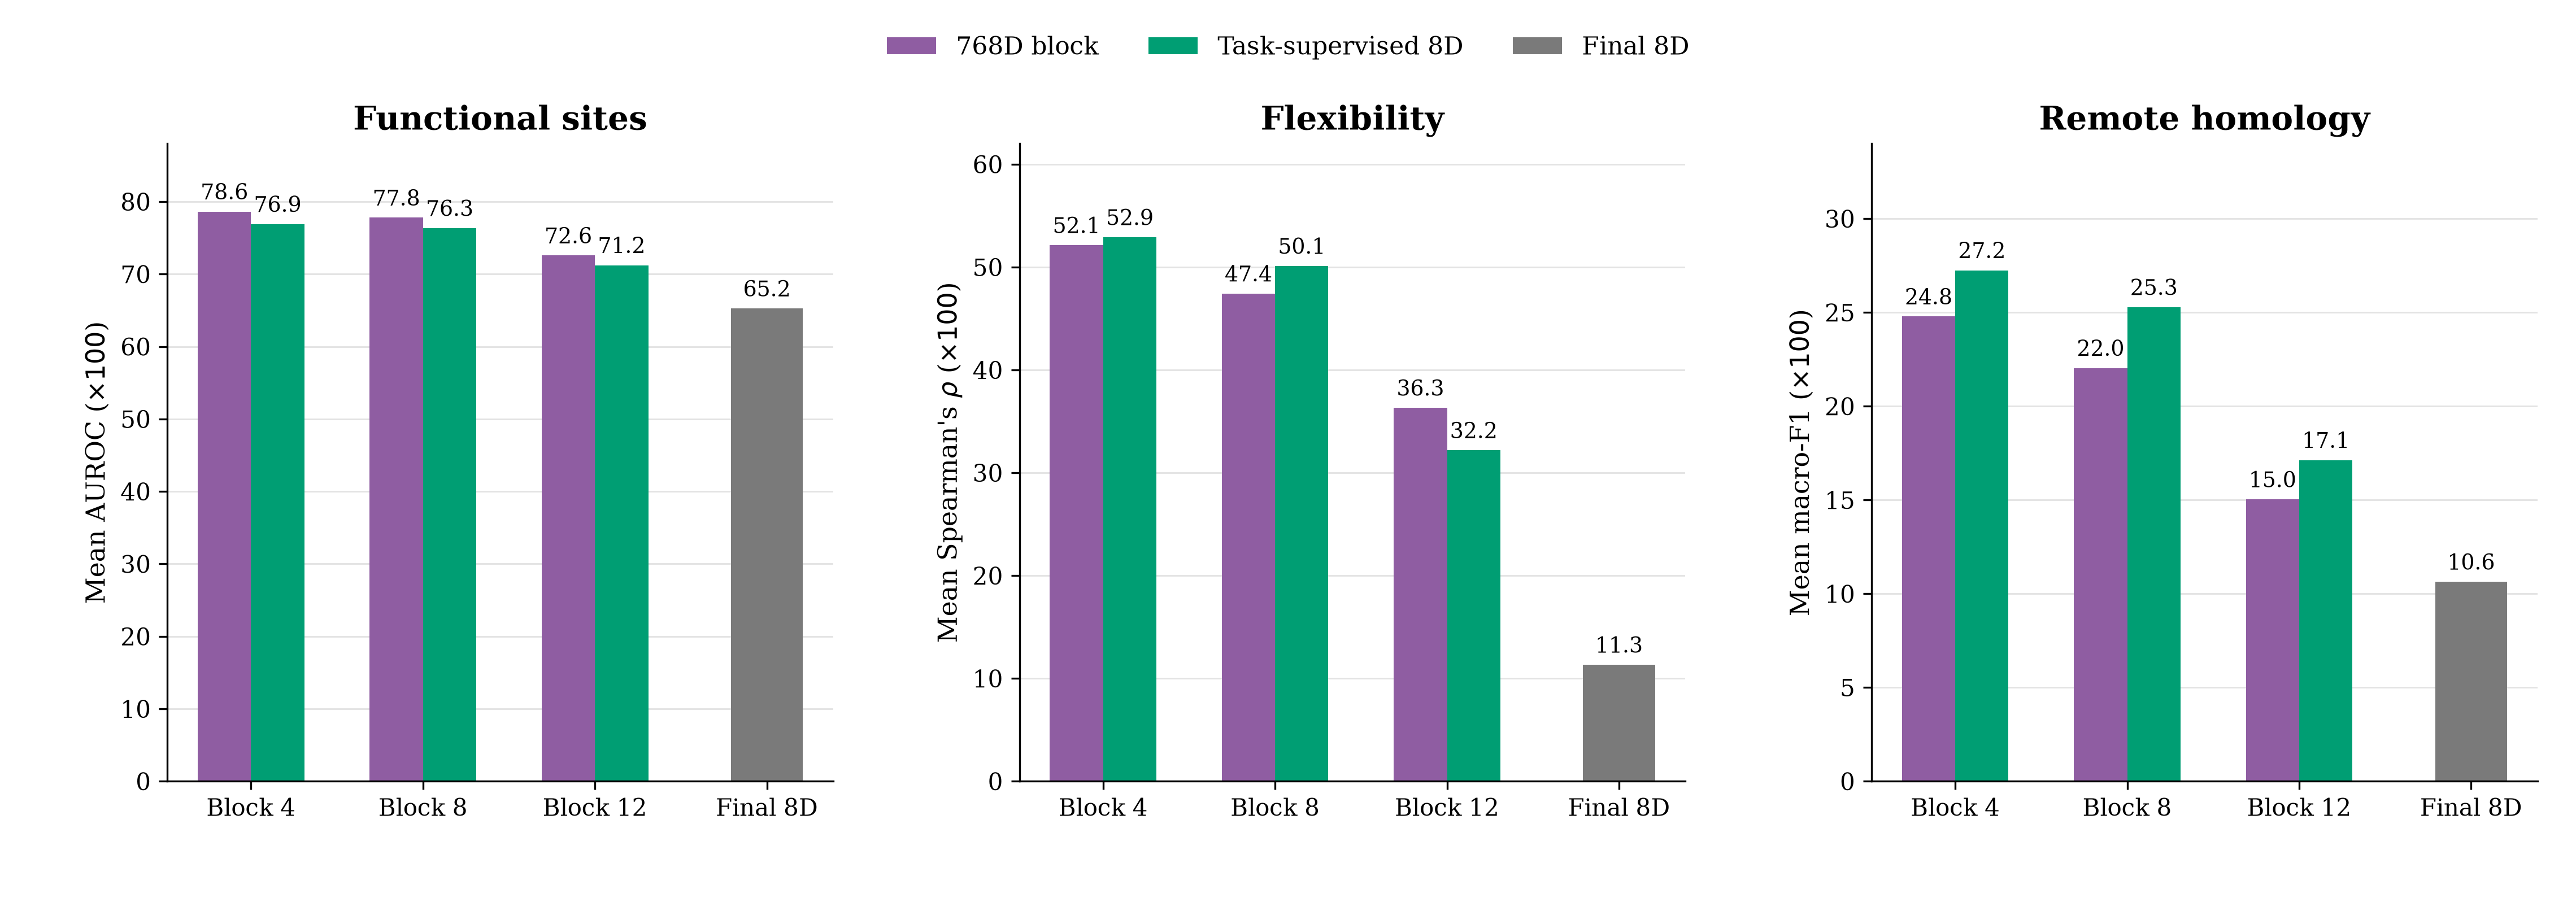
\includegraphics[width=0.78\linewidth]{canonical_lejepa_raw100k_supervised_bottleneck8_comparison.png}
  \caption{Frozen block representations compared with task-supervised 8D bottlenecks. Scores are multiplied by 100. Each downstream task learns its own 768D-to-8D projection, so this tests whether eight dimensions can retain information selected for that task. It is not a universal shared 8D representation. Light-purple bars show task-supervised 8D representations and blue bars show the encoder's final 8D latent.}
  \label{fig:bottleneck}
\end{figure}

\subsection{Layerwise replication in JEPA}

\begin{table}[!htbp]
\centering
\setlength{\tabcolsep}{4pt}
\renewcommand{\arraystretch}{0.82}
\fontsize{7.4}{8.4}\selectfont
\caption{Complete layerwise StructTokenBench results for JEPA with 70\% random masking at 100k. Hidden-block representations are 768D and the final representation is 8D. Scores are multiplied by 100, and bold marks the highest score in each row.}
\label{tab:jepa-r70-layerwise}
\begin{tabular}{@{}llrrrr@{}}
\toprule
Task & Split & Block 1 & Block 6 & Block 12 & Final 8D \\
\midrule
\multicolumn{6}{c}{\textbf{Functional-site prediction: AUROC $\times100$}} \\
\midrule
\multirow{2}{*}{BindInt} & Fold & 47.86 & \textbf{48.86} & 48.24 & 47.11 \\
 & SF & 88.24 & \textbf{91.95} & 91.59 & 80.06 \\
\multirow{2}{*}{BindBio} & Fold & 72.61 & \textbf{73.22} & 72.84 & 65.56 \\
 & SF & 72.93 & \textbf{73.85} & 73.76 & 65.31 \\
BindShake & Test & 78.23 & 78.13 & \textbf{78.38} & 71.85 \\
\multirow{2}{*}{CatInt} & Fold & 65.69 & \textbf{65.72} & 65.05 & 56.84 \\
 & SF & 88.00 & 91.79 & \textbf{92.00} & 76.71 \\
\multirow{2}{*}{CatBio} & Fold & \textbf{80.72} & 80.13 & 78.23 & 71.50 \\
 & SF & 89.81 & 89.62 & \textbf{90.39} & 75.36 \\
\multirow{2}{*}{Con} & Fold & 64.20 & \textbf{64.35} & 63.30 & 60.44 \\
 & SF & 80.83 & 84.74 & \textbf{85.64} & 72.08 \\
\multirow{2}{*}{Rep} & Fold & 74.11 & 75.90 & \textbf{76.03} & 73.77 \\
 & SF & 80.24 & 81.69 & \textbf{82.65} & 78.46 \\
\multirow{2}{*}{Ept} & Fold & \textbf{55.44} & 51.02 & 53.69 & 47.87 \\
 & SF & 66.56 & 68.70 & \textbf{70.50} & 49.29 \\
\midrule
\multicolumn{6}{c}{\textbf{Remote homology: macro-F1 $\times100$}} \\
\midrule
\multirow{3}{*}{Homo} & Fold & 6.57 & \textbf{12.86} & 12.25 & 9.86 \\
 & Family & 18.02 & \textbf{27.80} & 23.47 & 13.30 \\
 & SF & 7.43 & \textbf{14.69} & 11.42 & 6.00 \\
\midrule
\multicolumn{6}{c}{\textbf{Structural flexibility: Spearman's $\rho\times100$}} \\
\midrule
\multirow{2}{*}{FlexRMSF} & Fold & 45.27 & \textbf{53.17} & 53.11 & 33.98 \\
 & SF & 45.35 & 54.75 & \textbf{55.17} & 34.26 \\
\multirow{2}{*}{FlexBFactor} & Fold & \textbf{32.79} & 31.29 & 32.17 & 23.29 \\
 & SF & 26.88 & 27.47 & \textbf{28.42} & 21.69 \\
\multirow{2}{*}{FlexNEQ} & Fold & 19.24 & \textbf{37.63} & 34.59 & 25.11 \\
 & SF & 18.64 & \textbf{37.61} & 35.23 & 25.19 \\
\bottomrule
\end{tabular}
\end{table}
\end{document}
